%%%%%%%%%%%%%%%%%%%%%%%%%%%%%%%%%%%%%%%%%%%%%%%%%%%%%%%%%%%%%%%%%%%%%%%%%
%                           Marco Conceptual                               %
%%%%%%%%%%%%%%%%%%%%%%%%%%%%%%%%%%%%%%%%%%%%%%%%%%%%%%%%%%%%%%%%%%%%%%%%%

\chapter{Desarrollo del Sistema}\label{chapter5}

En este capitulo se cubre el desarrollo del sistema descrito en capítulos anteriores tomando como referencia los casos de uso, abarcando cada uno de los módulos que lo componen.

\section{Módulo del Microcontrolador}

\subsection{Objetivo}
Implementar los casos de uso \ref{SUB-M-CU1.1} (SUB-M-CU1.1) y \ref{SUB-M-CU1.2} (SUB-M-CU1.2), que nos indican que el microcontrolador debe consultar el dispositivo de adquisición MCP39F521 para conseguir el valor de potencia activa por medio del protocolo IIC y enviar esta información hacia el servidor embebido por medio del módulo WiFi, para lograr estas tareas, nos apoyamos en las hojas de datos de los fabricantes, debemos programar el microcontrolador DSPIC30F4013, para ello ocupamos el entorno de desarrollo del fabricante (mplab de Microchip) para crear un proyecto en lenguaje C y ensamblador, el entorno de desarrollo de microchip facilita la programación de sus microcontroladores gracias a que tiene bibliotecas y compiladores listos para usarse.

\subsection{Configurando la comunicación con el dispositivo de adquisición}
Lo primero que debemos conocer es como configurar la comunicación IIC del dispositivo de adquisición, el registro de control de IIC en el microcontrolador podemos encontrarlo en su hoja técnica (Página 89) \citep{DatasheetDSPIC30F4013}, el registro de control, entre sus funciones, habilita la comunicación IIC y configura la velocidad del reloj IIC, en la hoja técnica del dispositivo de adquisición nos indica que esta frecuencia es de 400KHz (Página 1) \citep{DatasheetDSPIC30F4013} y por lo tanto el microcontrolador debe trabajar a esta velocidad para poder lograr la comunicación, recordando que es un protocolo de transmisión de información síncrona por el uso de una linea de reloj.

\paragraph{}
Una ves configurada la comunicación, físicamente solamente necesitamos interconectar los pines de SDA (linea de datos), SCL (linea de reloj), VCC y GND de microcontrolador con dispositivo, este dispositivo ya contiene en sus registros los valores de potencia, voltaje y corriente entre otros que se pueden encontrar en el mapa de registros \ref{fig:Mapa de registros del MCP39F521}, que son convertidos y acondicionados automáticamente con el ADC y Filtro Digital que tiene ya integrado \ref{fig:Diagrama funcional} .

\begin{figure}[H]
	\centering
	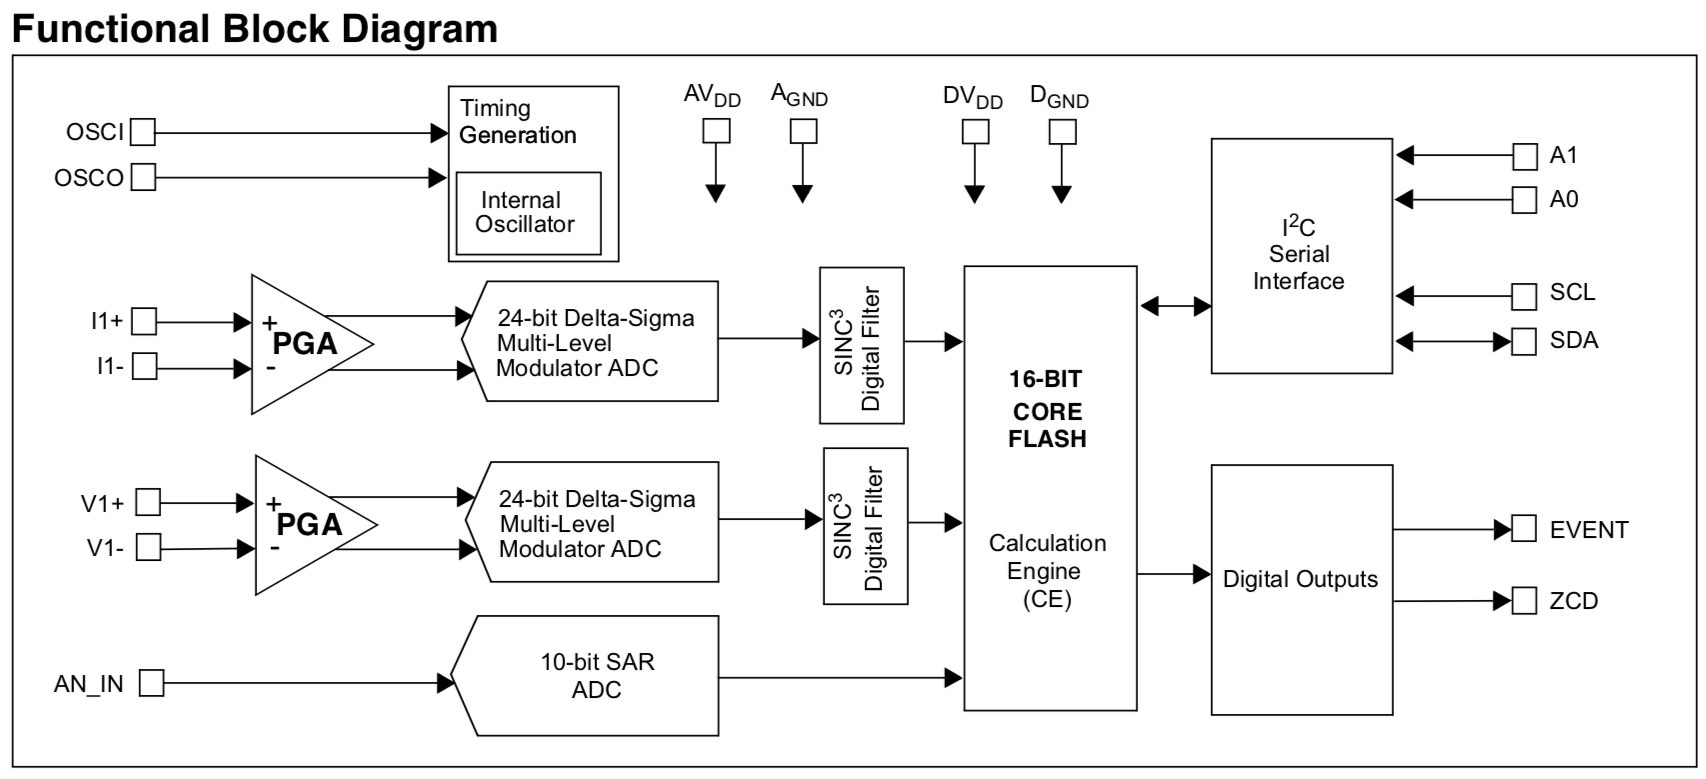
\includegraphics[scale=.4]{Capitulo5/images/MCP_diagrama_funcional.png}
	\caption{Diagrama funcional del dispositivo de adquisición}
	\label{fig:Diagrama funcional}
\end{figure}

\begin{figure}[H]
	\centering
	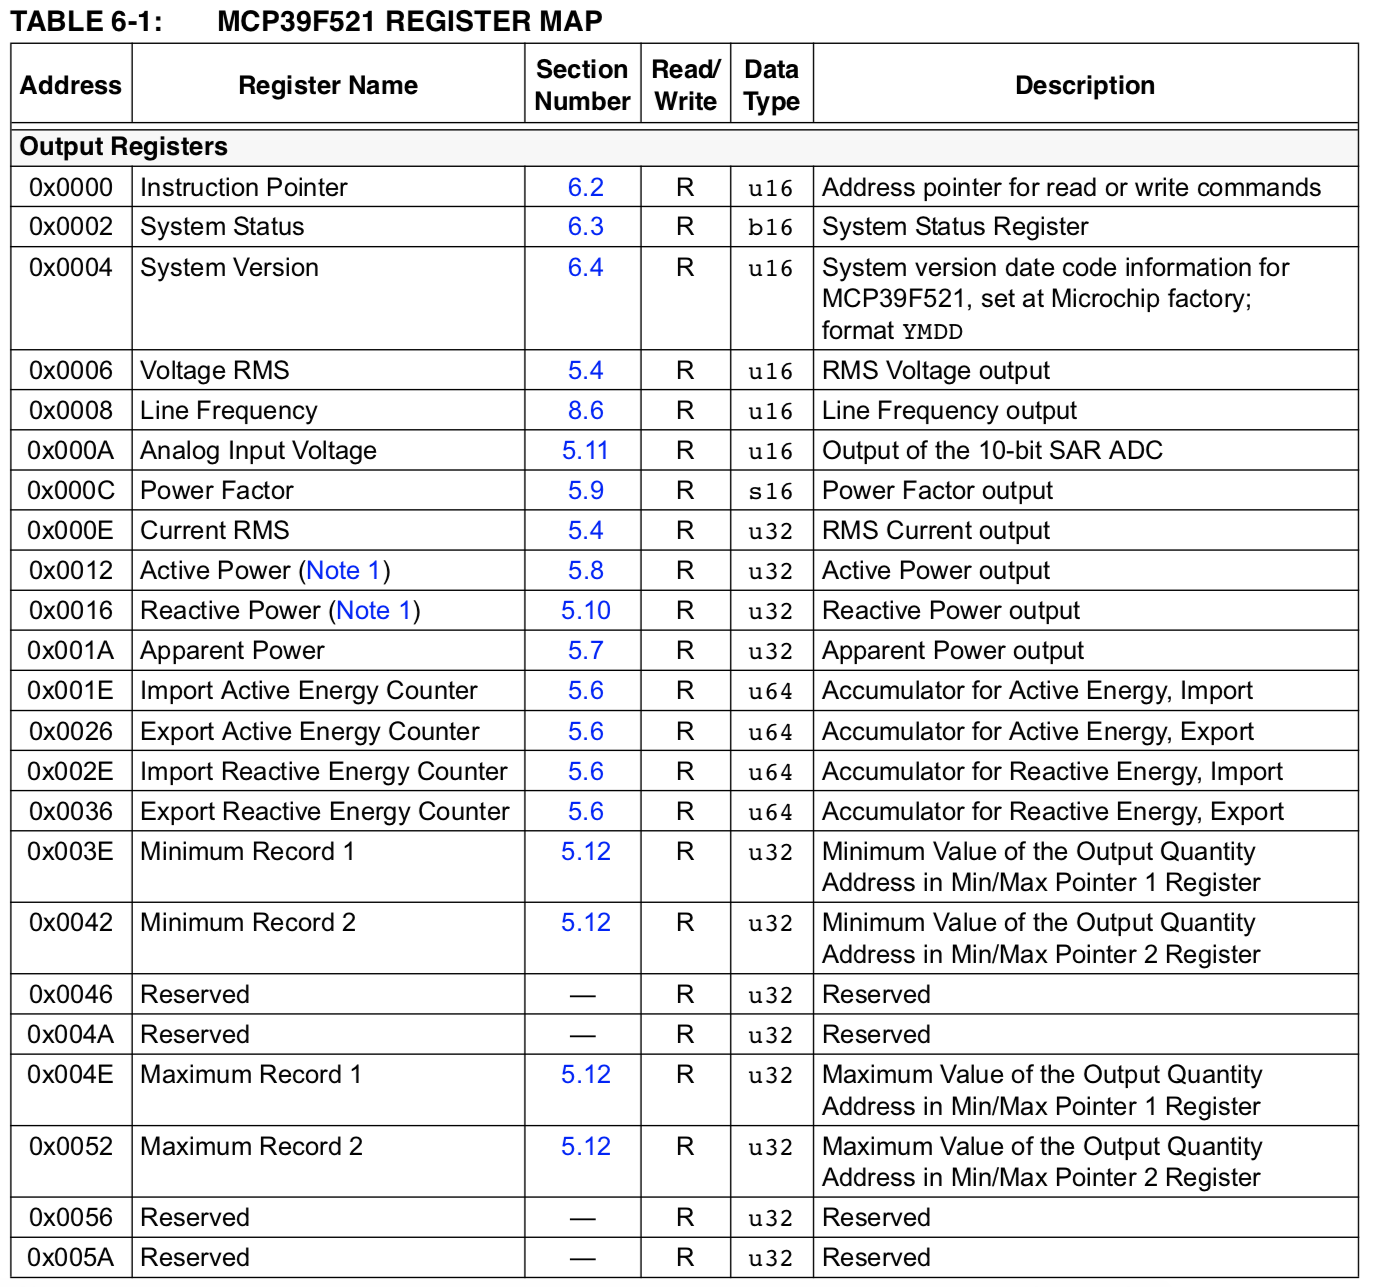
\includegraphics[scale=.5]{Capitulo5/images/register_map.png}
	\caption{Mapa de registros del MCP39F521}
	\label{fig:Mapa de registros del MCP39F521}
\end{figure}

\subsection{Comunicación con el dispositivo de adquisición vía software}

La comunicación IIC con el dispositivo de adquisición a nivel software se realiza, principalmente con los siguientes comandos definidos por el protocolo:

\begin{enumerate}
    \item Inicio de comunicación (START)
    \item Fin de comunicación (STOP)
    \item Acuse de recibo (ACK)
    \item No acuse de recibo (NACK)
    \item Envió de información
    \item Recibo de información
\end{enumerate}

Estas funciones ya están implementadas en lenguaje ensamblador, en una biblioteca denominada I2C.s y nosotros las ocupamos en el programa principal en lenguaje C por medio de su declaración global, en el código siguiente se muestran las rutinas para el comando de inicio de comunicación y envió de datos.

\begin{lstlisting}[language={[x86masm]Assembler}]

;****DECLARACION DE METODOS GLOBALMENTE PARA SU USO EN C*****
.GLOBAL	_START_I2C
.GLOBAL	_ENVIA_DATO_I2C

;************************************************************
ESTA RUTINA GENERA LA CONDICION DE START AL BUS I2C
ENVIANDO CON EL REGISTRO DE CONTROL AL ESCLAVO LA SEÑAL
Y ESPERANDO SU RESPUESTA
;************************************************************
_START_I2C:
	BCLR		IFS0,			#MI2CIF
	BSET		I2CCON,			#SEN
ESPERA_START:
	BTSS		IFS0,			#MI2CIF
	GOTO		ESPERA_START

	RETURN
	
;************************************************************
ESTA RUTINA GENERA LA CONDICION DE ENVIO DE DATO AL BUS I2C
EN ESTE CASO, COPIAMOS LO QUE ESTA EN EL REGISTRO W0 AL 
REGISTRO DE TRANSMISION DE I2C ESPERANDO LA RESPUESTA DEL
ESCLAVO
;************************************************************
_ENVIA_DATO_I2C:
	BCLR		IFS0,			#MI2CIF
	MOV.B		WREG,			I2CTRN
ESPERA_ENVIA_DATO_I2C:
	BTSS		IFS0,			#MI2CIF
	GOTO		ESPERA_ENVIA_DATO_I2C
	
	RETURN
	
\end{lstlisting}

\subsection{Escritura de comandos para el dispositivo de adquisición}

En la figura \ref{fig:Comando de escritura} se muestra la estructura de un byte de control para la escritura de un comando, contiene un bit de inicio, un byte de control que indica hacia qué dispositivo nos dirigiremos, A1 y A0 son los bits de direccionamiento, podemos dirigirnos hacia 4 diferentes dispositivos esclavos, en este caso al tener solo uno, la dirección será “00”, seguido del bit que indica si será una operación de lectura o escritura, al ser escritura toma el valor de cero, formando como byte de control “11101000”.

\begin{figure}[H]
	\centering
	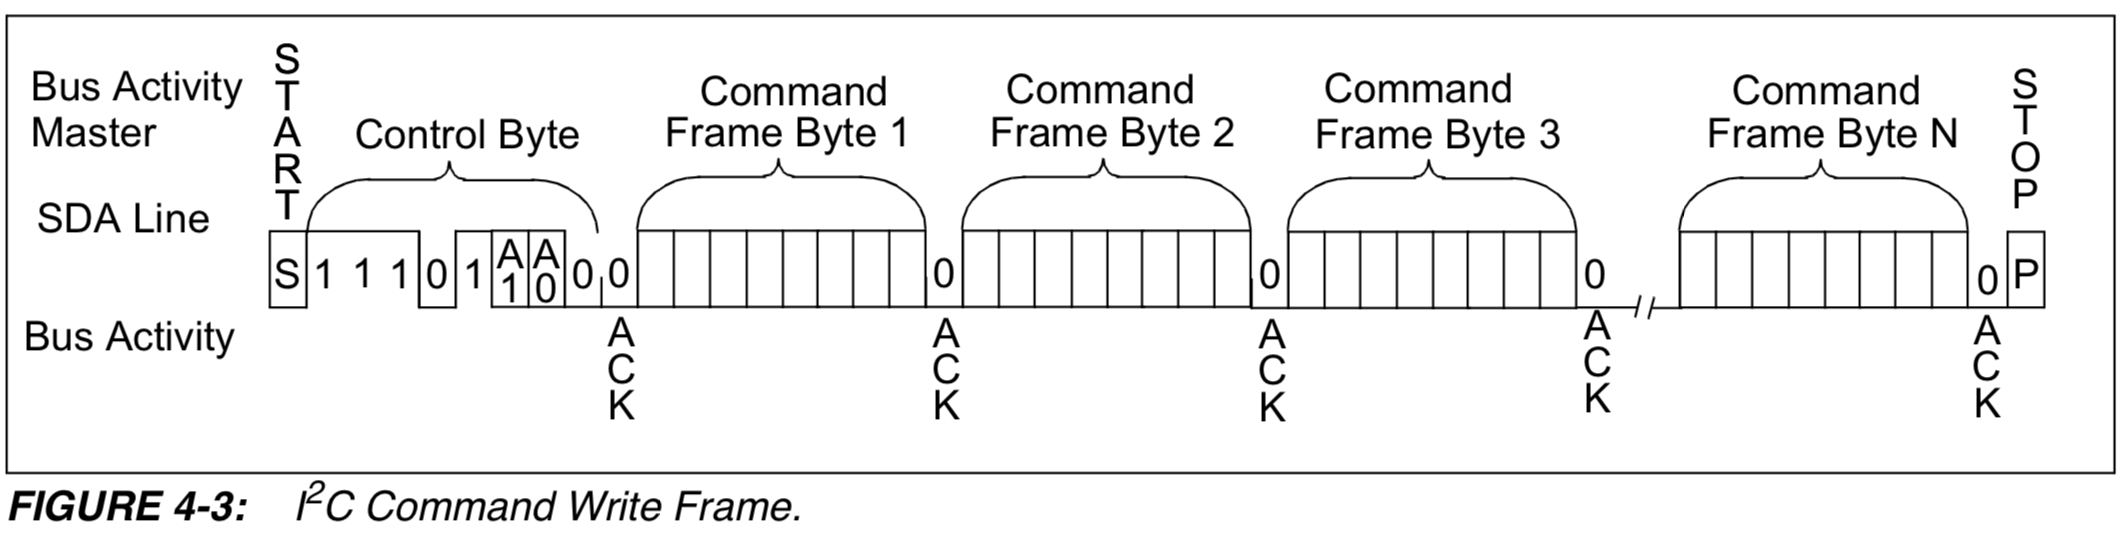
\includegraphics[scale=.4]{Capitulo5/images/write_command.png}
	\caption{Comando de escritura de comando para el dispositivo de adquisición MCP39F521}
	\label{fig:Comando de escritura}
\end{figure}

Este byte de control, indica al dispositivo de adquisición que vamos a iniciar una lectura, este es seguido por un marco o marcos de comandos a ejecutar como se muestra en la figura \ref{fig:Marco de escritura de lectura} , están compuestos por una cabecera, cuantos bytes se recibirán, el o los comandos a ejecutar y un checksum para verificar que la información llego completa y correcta, éste se calcula sumando los datos descritos y dividiéndolos entre 256, el residuo de esta división es el checksum.

\begin{figure}[H]
	\centering
	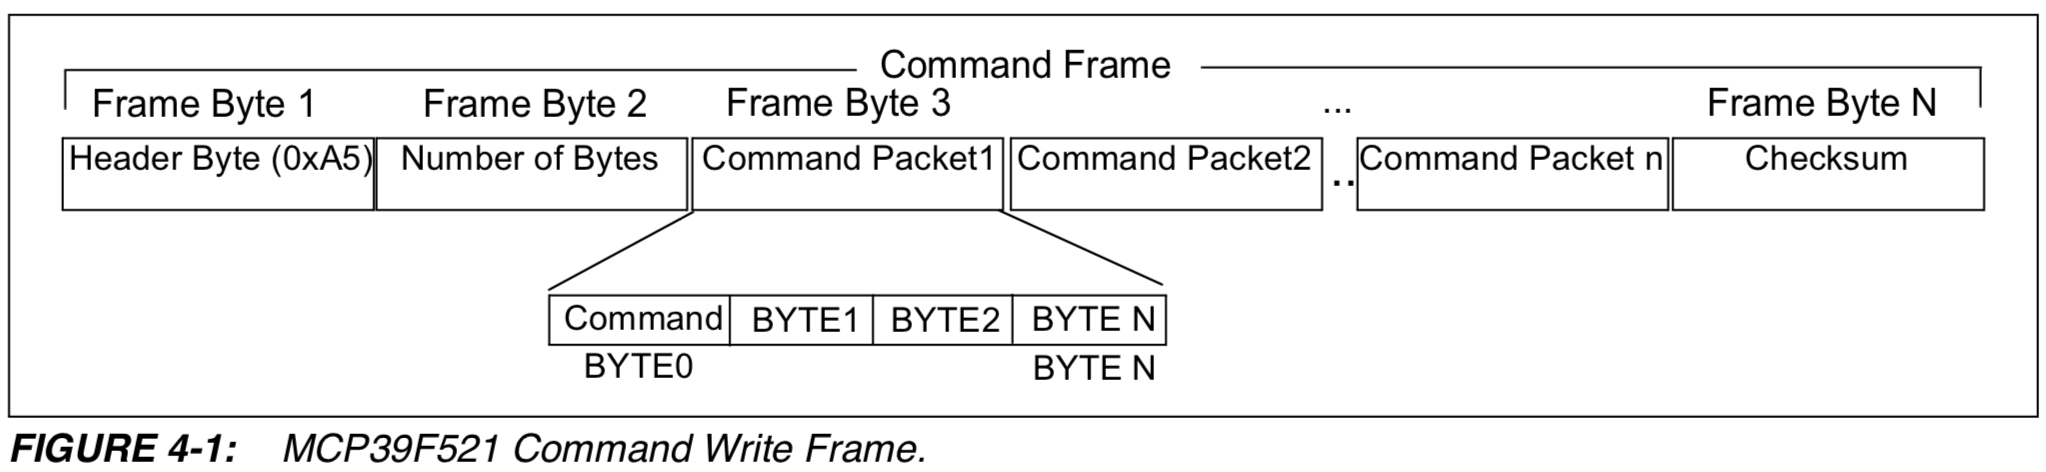
\includegraphics[scale=.4]{Capitulo5/images/marco_write_command.png}
	\caption{Marco para la escritura de un comando de lectura}
	\label{fig:Marco de escritura de lectura}
\end{figure}

Traducido a código en lenguaje c, la rutina que escribe un comando de lectura de registro se ve de la siguiente forma:

\begin{lstlisting}[language=C]

unsigned char enviaComando ( 
  unsigned char direccion, unsigned char registro, 
  unsigned char bytes, unsigned char checksum )
{
    START_I2C();
 
    //Control byte, write command
    
    ENVIA_DATO_I2C(direccion); //11101000   
    
    if( I2CSTATbits.ACKSTAT == 1 ){ //NACK del sensor
        return NANCK;
    }

    // Inicio del I2C Command Write Frame.
    
    ENVIA_DATO_I2C(0xA5); //header byte
        
    ENVIA_DATO_I2C(0x08); //no. bytes in frame
    
    ENVIA_DATO_I2C(0x41); //command set address pointer
   
    ENVIA_DATO_I2C(0x00); //addr high
     
    ENVIA_DATO_I2C(registro); //addr low 

    ENVIA_DATO_I2C(0x4E); //command read register
    
    ENVIA_DATO_I2C(bytes); //number of bytes to read 
    
    ENVIA_DATO_I2C(checksum); //checksum   
   
    if( I2CSTATbits.ACKSTAT == 1 ){ //NACK del sensor
        return NANCK;
    }
          
    STOP_I2C();
    return EXITO;
}

\end{lstlisting}

Por ejemplo, si queremos conocer el valor de la frecuencia, debemos mandar con la función definida, la señal de inicio de comunicación START y el byte de control de escritura hacia el sensor cero (0xE8), esperar a recibir el acuse de recibo (ACK), enviar la cabecera del marco (A5), el número de bytes que tendrá el marco (contando desde la cabecera hasta el checksum: 0x08), la dirección del registro a leer del mapa, separado en la parte alta y baja (0x00 , 0x08), el comando de lectura de registro (0x4E), el número de bytes a leer, el registro de voltaje tiene una longitud de dos bytes (0x02) y el checksum (0x46), sumado desde el byte de cabecera del marco (0x44) por ultimo, recibiremos el acuse de recibo (ACK) y terminamos la comunicación con un STOP:

\paragraph{}
\framebox[\linewidth]{START() 0xE8 ACK() 0xA5 0x08 0x41 0x00 0x08 0x4E 0x02 0x46 ACK() STOP()}\par

\subsection{Lectura de respuesta del dispositivo de adquisición}

Ahora que logramos comunicarnos con el sensor para requerir la lectura de su o sus registros, necesitamos conocer la respuesta resultante, para ello tenemos que seguir el formato del byte de control de lectura de respuesta del dispositivo esclavo como el fabricante indica y se muestra en la figura \ref{fig:Comando de lectura de respuesta} , tiene un bit de inicio, un byte de control, que nos indica a qué dispositivo esclavo nos dirigimos, en este caso una vez más al “00”, seguido del bit que indica si será una operación de lectura o escritura, al ser lectura toma el valor de uno, formando como byte de control “11101001” seguido de los marcos de respuesta.

\begin{figure}[H]
	\centering
	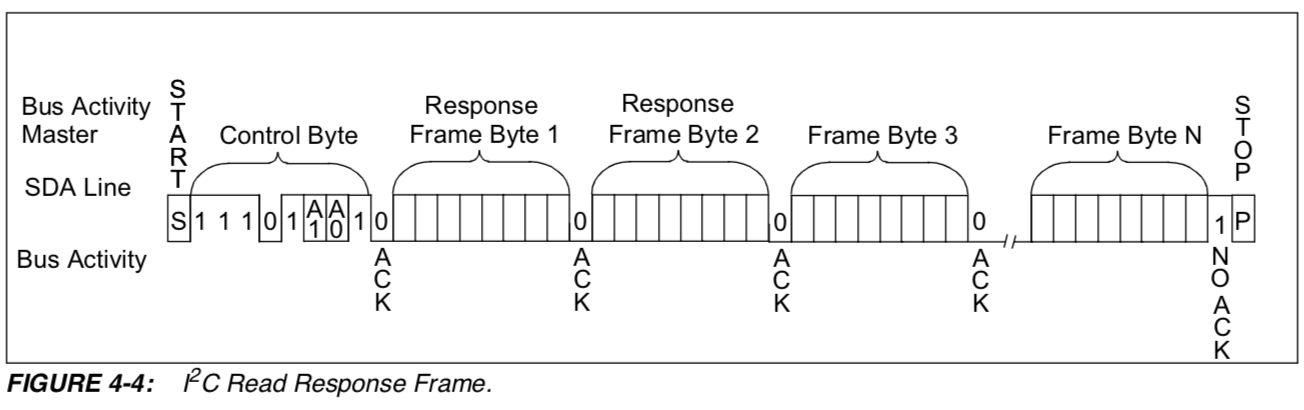
\includegraphics[scale=.7]{Capitulo5/images/read_command.png}
	\caption{Comando de lectura para el dispositivo de adquisición MCP39F521}
	\label{fig:Comando de lectura de respuesta}
\end{figure}

Después del envió del byte de control, recibimos los marcos de respuesta que se muestran en la figura \ref{fig:Marco de respuesta} , que nos indican un acuse especial con valor de 6 hexadecimal, seguido de el numero de bytes que lo conforman, los bytes de información y finalmente un checksum.

\begin{figure}[H]
	\centering
	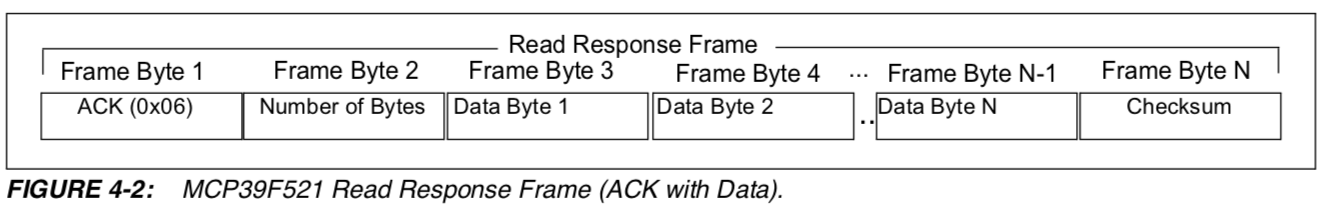
\includegraphics[scale=.7]{Capitulo5/images/responde_frame.png}
	\caption{Marco de respuesta para el dispositivo de adquisición MCP39F521}
	\label{fig:Marco de respuesta}
\end{figure}

Traducido a código en lenguaje c, la rutina que escribe un comando de lectura de respuesta se ve de la siguiente forma:

\begin{lstlisting}[language=C]

unsigned char leeRespuesta(unsigned char direccion)
{   
    
    START_I2C();
    
    //control byte, read response
    
    ENVIA_DATO_I2C(direccion+0x01); //11101001   
    
    if( I2CSTATbits.ACKSTAT == 1 ){ //NACK del sensor
        return NANCK;
    }

    //ack (0x06)
    RECIBE_DATO_I2C();
    ACK_MST_I2C();
    
    //number of bytes 
    int no_bytes = RECIBE_DATO_I2C();
    ACK_MST_I2C();
    
    int i;
    
    //data bytes
    for(i = 0 ; i < no_bytes-3 ; i++){
        U2TXREG = RECIBE_DATO_I2C();
        ACK_MST_I2C();
    }
    
    //checksum
    RECIBE_DATO_I2C();
    NACK_MST_I2C();
    
    STOP_I2C();  
    return EXITO;
}

\end{lstlisting}


Por ejemplo, si queremos leer la respuesta a la lectura del registro de frecuencia, se envia la señal de inicio de comunicación START y el byte de control de lectura hacia el dispositivo cero (0xE9), esperar a leer el acuse de recibo (ACK), el numero de bytes que se reciben del dispositivo esclavo, al valor que se recibe se restan tres bytes: acuse, checksum y numero de bytes (0x05). A continuación de reciben los bytes de datos (0x66 , 0xEA) que finalizan con un checksum y terminamos la comunicación con un STOP:

\paragraph{}
\framebox[\linewidth]{START() 0xE9 ACK() 0x05 0x66 0xEA 0x55 ACK() STOP()}\par

\subsection{Envío de muestras al servidor vía Wi-Fi}

Con estas éstas dos rutinas, conseguimos en bytes, la información de los registros que requiramos con el comando de lectura de registro, para nuestro caso, traeremos el valor del voltaje, corriente, factor de potencia, frecuencia, potencia aparente, activa y reactiva de un panel solar, estos bytes los enviamos por medio del módulo Wi-Fi por medio de la interfaz de comunicación UART, la conexión física de este módulo Wi-Fi es sencilla, usa un estándar de pines para su montura llamado mikrobus (\ref{fig:Mikrobus}), que principalmente tiene un transmisor (TX), receptor (RX), ChipSelect (CS) así como GND y VCC. 

\begin{figure}[H]
	\centering
	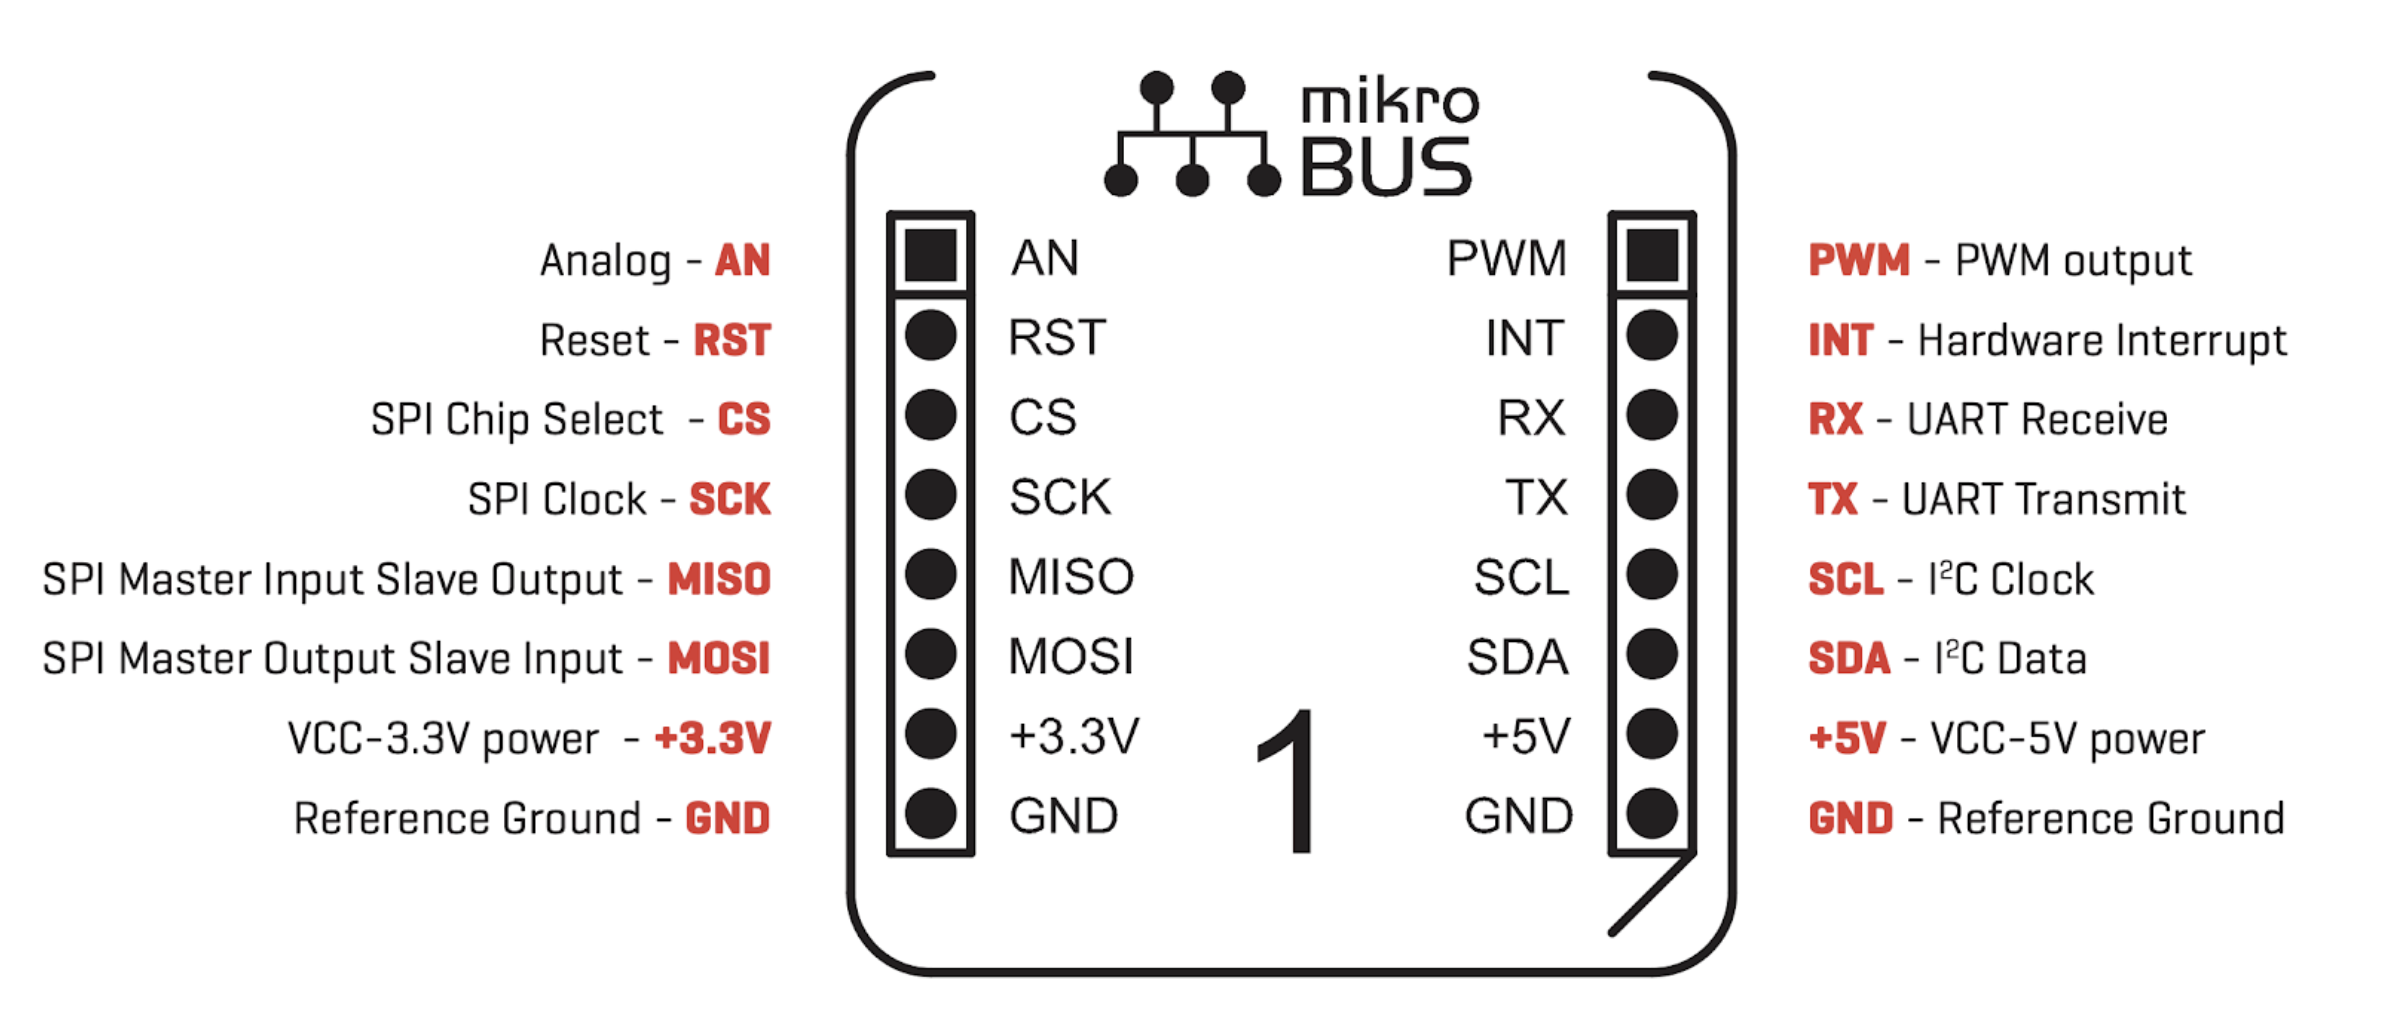
\includegraphics[scale=.2]{Capitulo2/images/mikrobus.png}
	\caption{Estándar de Pines Mikrobus}
	\label{fig:Mikrobus}
\end{figure}

Para poder usar el modulo WiFi a nivel programación, debemos primero, configurar los registros de configuración del modulo UART, el MCP30F4013 tiene 2 interfaces UART, pero la segunda es la que tiene el acomodo para el estándar mikrobus, debemos activar la interfaz UART por medio de su registro de configuracion en el microcontrolador, configurar la velocidad de transición de información, esto se calcula dividiendo la frecuencia de trabajo de nuestro microcontrolador (1.8 MHz) entre el Baudaje del módulo Wi-FI, que es de 115200 Baudios.

Después, debemos configurar la interrupción del transmisor UART, de manera que cuando se reciba un dato en el registro receptor, podamos proseguir con otras operaciones sin tener que retardar el proceso de configuracion o envío.

\begin{lstlisting}[language=C]

void iniprograma(){
    
    CONTRX = 0;
    
    iniPerifericos();
    
    //UART2 BAUDIOS:115200 mikrobus2 (WIFI)
    U2MODE = 0X0020; //uart disable ,no usa los alternos, autobaudaje
    U2STA  = 0X8000;
    U2BRG  = 0; // (1.8432*10^6)/(16*115200) = 0

    //Interrupciones de uart2 (Modulo wifi))
    IFS1bits.U2RXIF= 0;
    //U2RX interrupts ENABLE
    IEC1bits.U2RXIE= 1;
    
    //Habilitamos el uart2 (Modulo wifi)
    U2MODEbits.UARTEN = 1;
    U2STAbits.UTXEN = 1;
    
    //habilitando el registro de control sensor
    I2CCONbits.I2CEN = 1;
    
    //Inicializamos el modulo wifi
    iniWIFI();
    configWIFI();
}

\end{lstlisting}

Una vez configurada la comunicación UART con el módulo Wi-Fi, es configurar la red del mismo, esto se realiza con comandos AT, dónde configuramos la red a la que nos conectaremos, el protocolo de envió de paquetes, en este caso UDP, a que IP y Puerto nos dirigimos, donde indico la dirección del servidor y cuantos bytes de información se enviarán.

\begin{lstlisting}[language=C]
//Configuracion del modulo WIFI
void configWIFI(void){  
    
    comandoAT("ATE0\r\n"); //echo off
    sendOK();
    comandoAT("AT+RST\r\n");
    sendOK();
    comandoAT("AT+CWMODE=1\r\n"); //wifi-mode: softAP + station mode
    sendOK();
    comandoAT("AT+CIPMUX=0\r\n"); //disable multiple connections
    sendOK();
    comandoAT("AT+CWJAP=\"CELECSIS\",\"PIC18f2550\"\r\n");
    sendOK();
    comandoAT("AT+CIFSR\r\n"); //get local ip address 
}

//Envio de paquetes
void enviaWIFI(void){
    
    comandoAT("AT+CIPSTART=\"UDP\",\"104.198.212.166\",4000\r\n");
    sendOK();
    comandoAT("AT+CIPSEND=21\r\n");
    sendOK();
    
    //---Colocar aquí los nodos existentes---//
    
    //---Enviando numero de serie de microcontolador (AA)
    numero de sensor (0) y su informacion ---//
    U2TXREG = 'A';
    U2TXREG = 'A';

    U2TXREG = 0x00;

    leeTransmiteSensor(0xE8);
    sendOK();
    //----------------------------------------//   
    
    
    comandoAT("AT+CIPCLOSE\r\n");
    sendOK();
    
}
\end{lstlisting}

En la función principal, se envían muestras al servidor, no exactamente cada segundo, hicimos pruebas y cubre 50 muestras al minuto y hacemos un reinicio cada 30 minutos por si hay algún tipo de falla con la conexión de red.

\begin{lstlisting}[language=C]
//programa principal
int main (void)
{     
    iniprograma();

    //reinicio del programa cada media hora
    int counter = 0;
    
    //enviamos muestras cada segundo y reiniciamos el sistema cada media hora
    for(;EVER;)
    {           
        enviaWIFI();
        
        counter = counter+1;
        
        if(counter == 900){
            iniprograma();
            counter = 0;
        }
        
        __delay_ms(500);
    }
    
    return 0;
}
\end{lstlisting}

\subsection{Resultado final}

Físicamente, la figura \ref{fig:conexion hardware} muestra como se hace la conexión entre microcontrolador con dispositivo de adquisición, el montaje del modulo Wi-Fi, la conexión del panel solar a la carga y su inyección a la linea eléctrica.
    
\begin{figure}[H]
	\centering
	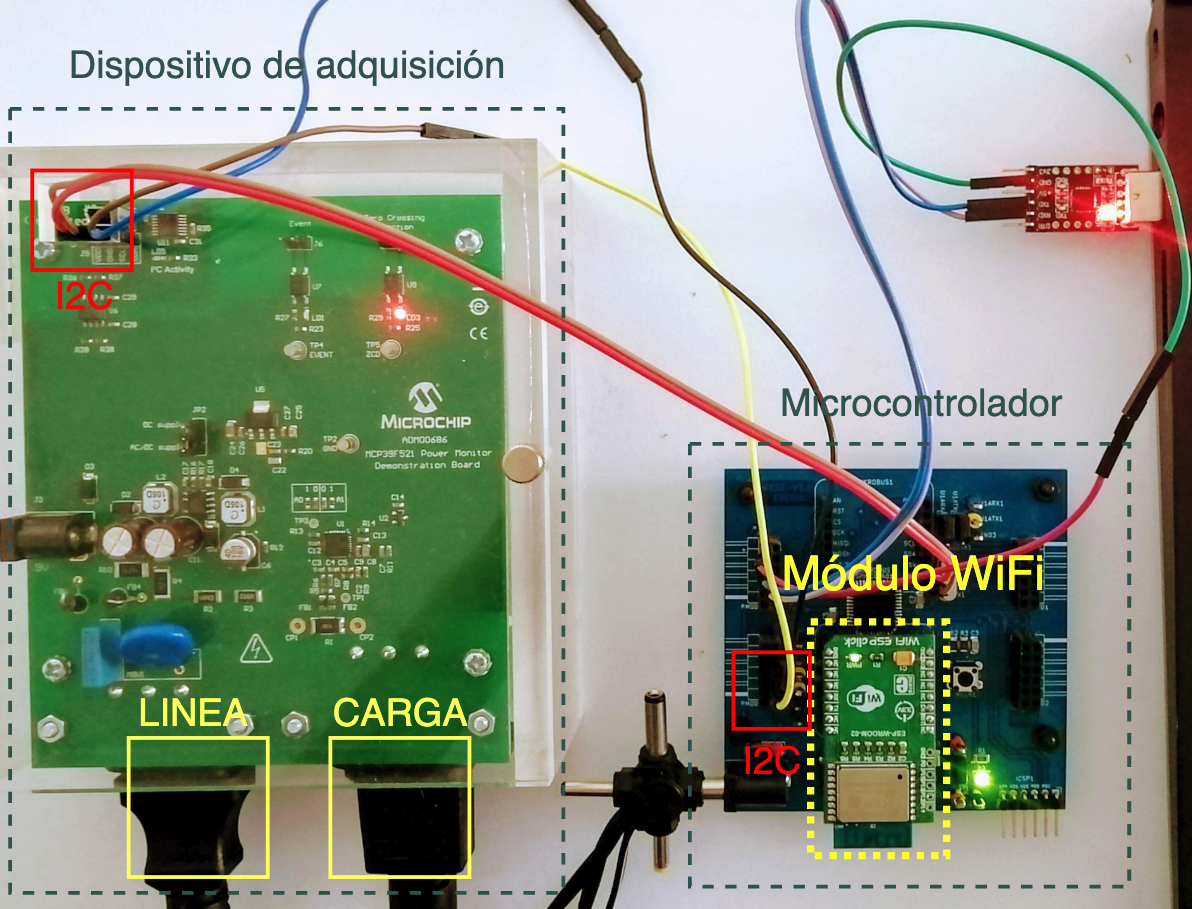
\includegraphics[scale=.3]{Capitulo5/images/conexion_fisica.png}
	\caption{Conexión de hardware del sistema}
	\label{fig:conexion hardware}
\end{figure} 

Para probar el funcionamiento de la comunicación con el dispositivo de adquisición via IIC, se conecto un cable USB con comunicación UART al microcontrolador, que copia los mismos datos que se envían al modulo Wi-Fi, a una computadora, solamente agregamos los pines del UART1 en la configuración del programa y copiamos en su registro de transmisión los datos conseguidos, nos basamos en el ejemplo de la hoja técnica para comparar el resultado conseguido.

\begin{figure}[H]
	\centering
	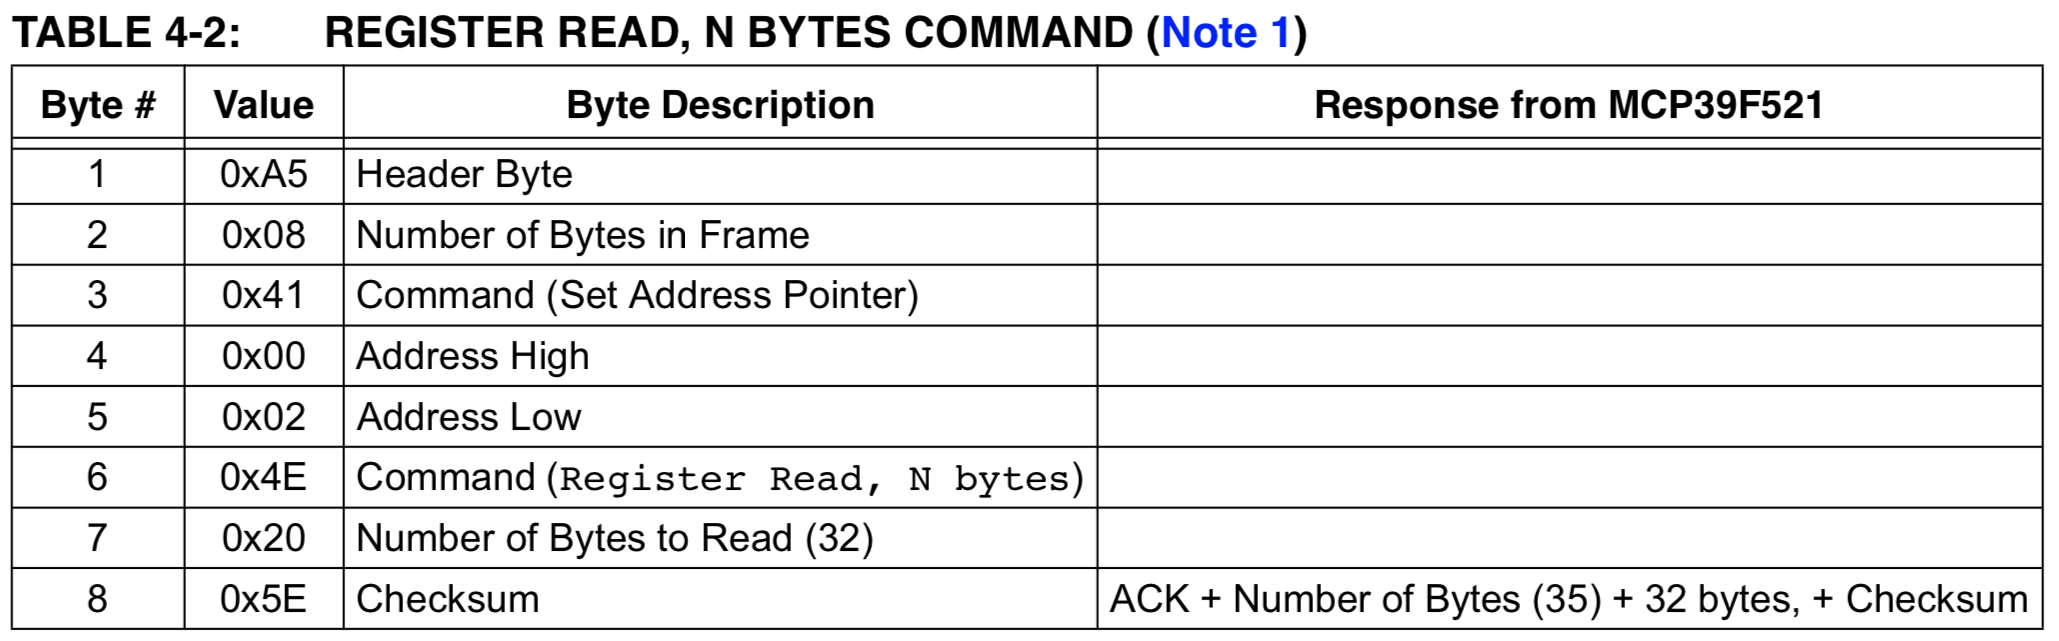
\includegraphics[scale=.3]{Capitulo5/images/respuesta_sensor.png}
	\caption{Respuesta del sensor a un comando de lectura determinado}
	\label{fig:respuesta sensor}
\end{figure} 

En la consola de la computadora, vemos la siguiente información impresa en pantalla,  podemos interpretarla de la siguiente forma:

\begin{itemize}
    \item Los dos primeros valores 255 nos marcan el fin de la transmisión
    \item ACK de la respuesta del esclavo (6 en ascii).
    \item Número de bytes (35)
    \item Los siguientes 32 datos son los datos enviados por el dispositivo esclavo del estado del sistema segun el mapa de registros \ref{fig:Mapa de registros del MCP39F521} .
    \item El 170 es el checksum del envío de la trama, podemos comprobarlo sumando desde el valor del acuse (6) hasta el penúltimo dato, dando un total de 1706 decimal, si dividimos esto entre 256, el valor del checksum será igual al residuo de la división, que es igual a 170.
\end{itemize}

\begin{figure}[H]
	\centering
	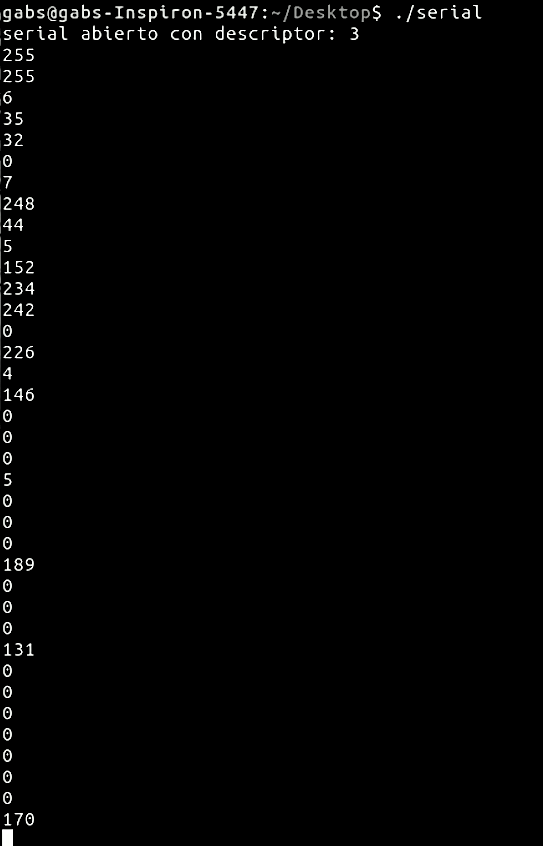
\includegraphics[scale=.3]{Capitulo5/images/consola.png}
	\caption{Respuesta proveniente del sensor a un comando de lectura de su registro}
	\label{fig:consola}
\end{figure} 

La ultima funcionalidad por probar es el envió de muestras al servidor, lo único que tenemos que hacer, es crear un servidor UDP en la IP y Puerto indicados en el programa del microcontrolador para la captura de los paquetes:


\begin{lstlisting}[language=Python]
import socket
import sys
import datetime, time
import os
import struct

#---------------Variables de configuracion-----------------
server_ip = '10.128.0.2'
port = 4000
#----------------------------------------------------------

# Creando socket UDP
sock = socket.socket(socket.SOCK_DGRAM, socket.SOCK_DGRAM)

# Relacionar direccion IP con puerto
server_address = (server_ip, port)
sock.bind(server_address)

print ('Starting up server on %s port %s' % server_address)

# Esperando por conexion
while True:

    print('Waiting for a connection...')
    
    pack, client_connection = sock.recvfrom(21)

    #Recibiendo paquete de 21 bytes
    pack = struct.unpack('21B',pack)

    packet = pack

    #Imprimir paquete recibido
    print(packet)

\end{lstlisting}

Y el resultado de este programa, es la captura de paquetes que tienen una longitud de 21 Bytes:
\begin{itemize}
    \item Byte 1 y 2: El numero de serie del microcontrolador en código ASCII.
    \item Byte 3: El numero de esclavo.
    \item Byte 4 y 5 : El valor del voltaje.
    \item Byte 6 y 7 : El valor de la frecuencia.
    \item Byte 8 y 9 : El valor de la corriente.
    \item Byte 10,11,12 y 13 : El valor de la potencia aparente.
    \item Byte 14,15,16 y 17 : El valor de la potencia activa.
    \item Byte 18,19,20 y 21 : El valor del factor de potencia.
\end{itemize}

Los valores que tienen mas de un byte, son enviados empezando por el byte menos significativo y terminando con el byte más significativo, esto es porque son valores decimales, a los bytes que se consiguen se les hace un corrimiento de bits para conseguir el valor original.
A continuación se muestra la captura de paquetes UDP procedentes del microcontrolador, cada paquete trae 21 bytes que se muestran en valor decimal en consola:

\begin{figure}[H]
	\centering
	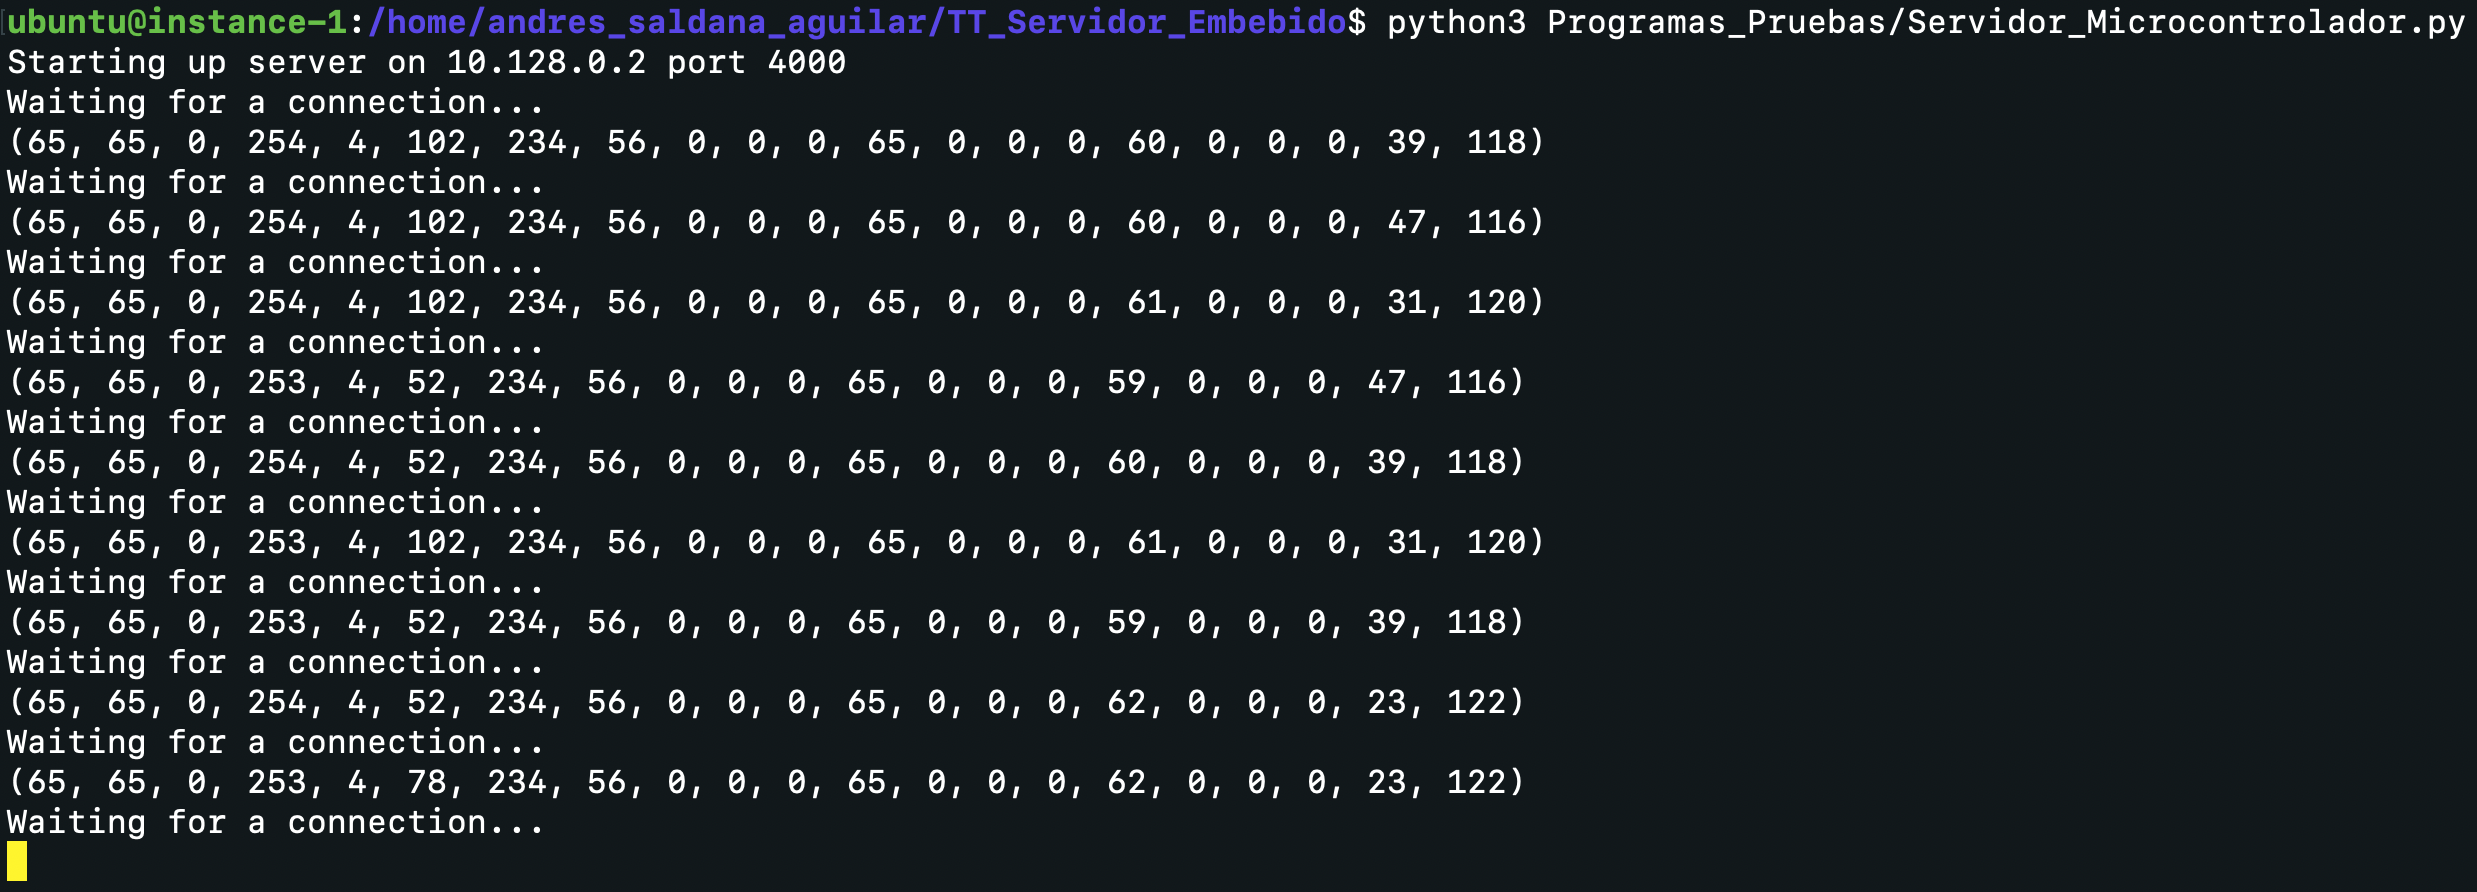
\includegraphics[scale=.3]{Capitulo5/images/paquetes_recibidos.png}
	\caption{Programa capturador de paquetes enviados por el microcontrolador en valor decimal}
	\label{fig:respuesta sensor}
\end{figure} 


De está manera se concluye la funcionalidad de la obtención y envió vía Wi-Fi de mediciones de potencia producida por un panel solar.

\section{Módulo del Servidor Embebido}

\subsection{Objetivo}
Implementar la funcionalidad descrita en los casos de uso \ref{SUB-M-CU1.3} (SUB-M-CU1.3), \ref{SUB-M-CU1.4} (SUB-M-CU1.4) y \ref{SUB-M-CU1.5} (SUB-M-CU1.5), dónde indicamos que nuestros servicios estarán alojados en un servidor web en el sistema embebido RaspBerry Pi 3. Los servicios que este ofrecerá son:

\begin{itemize}
    \item Configurar el entorno del servidor embebido
    \item Capturar y consumir paquetes UDP provenientes de los distintos microcontroladores para el calculo de producción de energía, monitoreo y gráficas \ref{SUB-M-CU1.3} (SUB-M-CU1.3).
    \item Consultar y almacenar cada minuto la generación de cada nodo \ref{SUB-M-CU1.5} (SUB-M-CU1.5).
    \item Atender a las peticiones de la aplicación móvil sobre la información de un nodo o de la red de sensores \ref{SUB-M-CU1.4} (SUB-M-CU1.4).
\end{itemize}

\subsection{Configurar el servidor embebido}

Utilizaremos el SBC Raspberry Pi 3 \citep{MarcoTeorico19} como servidor de aplicaciones y almacén de datos, para poder lograr esto, usaremos como sistema operativo Ubuntu Core de Linux, especialmente hecha para esta tarjeta, los pasos para cargar la imagen del sistema se describen en \citep{InstallUbuntuCore}, los pasos son:

\begin{itemize}
    \item Descargar la imagen de Ubuntu Core (2.42 GB) de la página oficial de Canonical.
    \item Formatear una memoria MicroSD (en nuestro caso con una capacidad de 16GB) y copiar en el la imagen de Ubuntu Core en él.
    \item Introducir la memoria en la ranura de la Raspberry Pi 3, conectar a el un cable Ethernet un teclado y monitor.
\end{itemize}

Para formatear la memoria, utilizamos la herramienta de MacOS de gestión de discos, que nos permite formatear volúmenes en el formato DOS FAT 32 que requiere la imagen, debemos asignarle un nombre al volumen que deberemos recordar para el siguiente paso, el resultado del formato se muestra en la figura \ref{fig:formato}.
 
\begin{figure}[H]
	\centering
	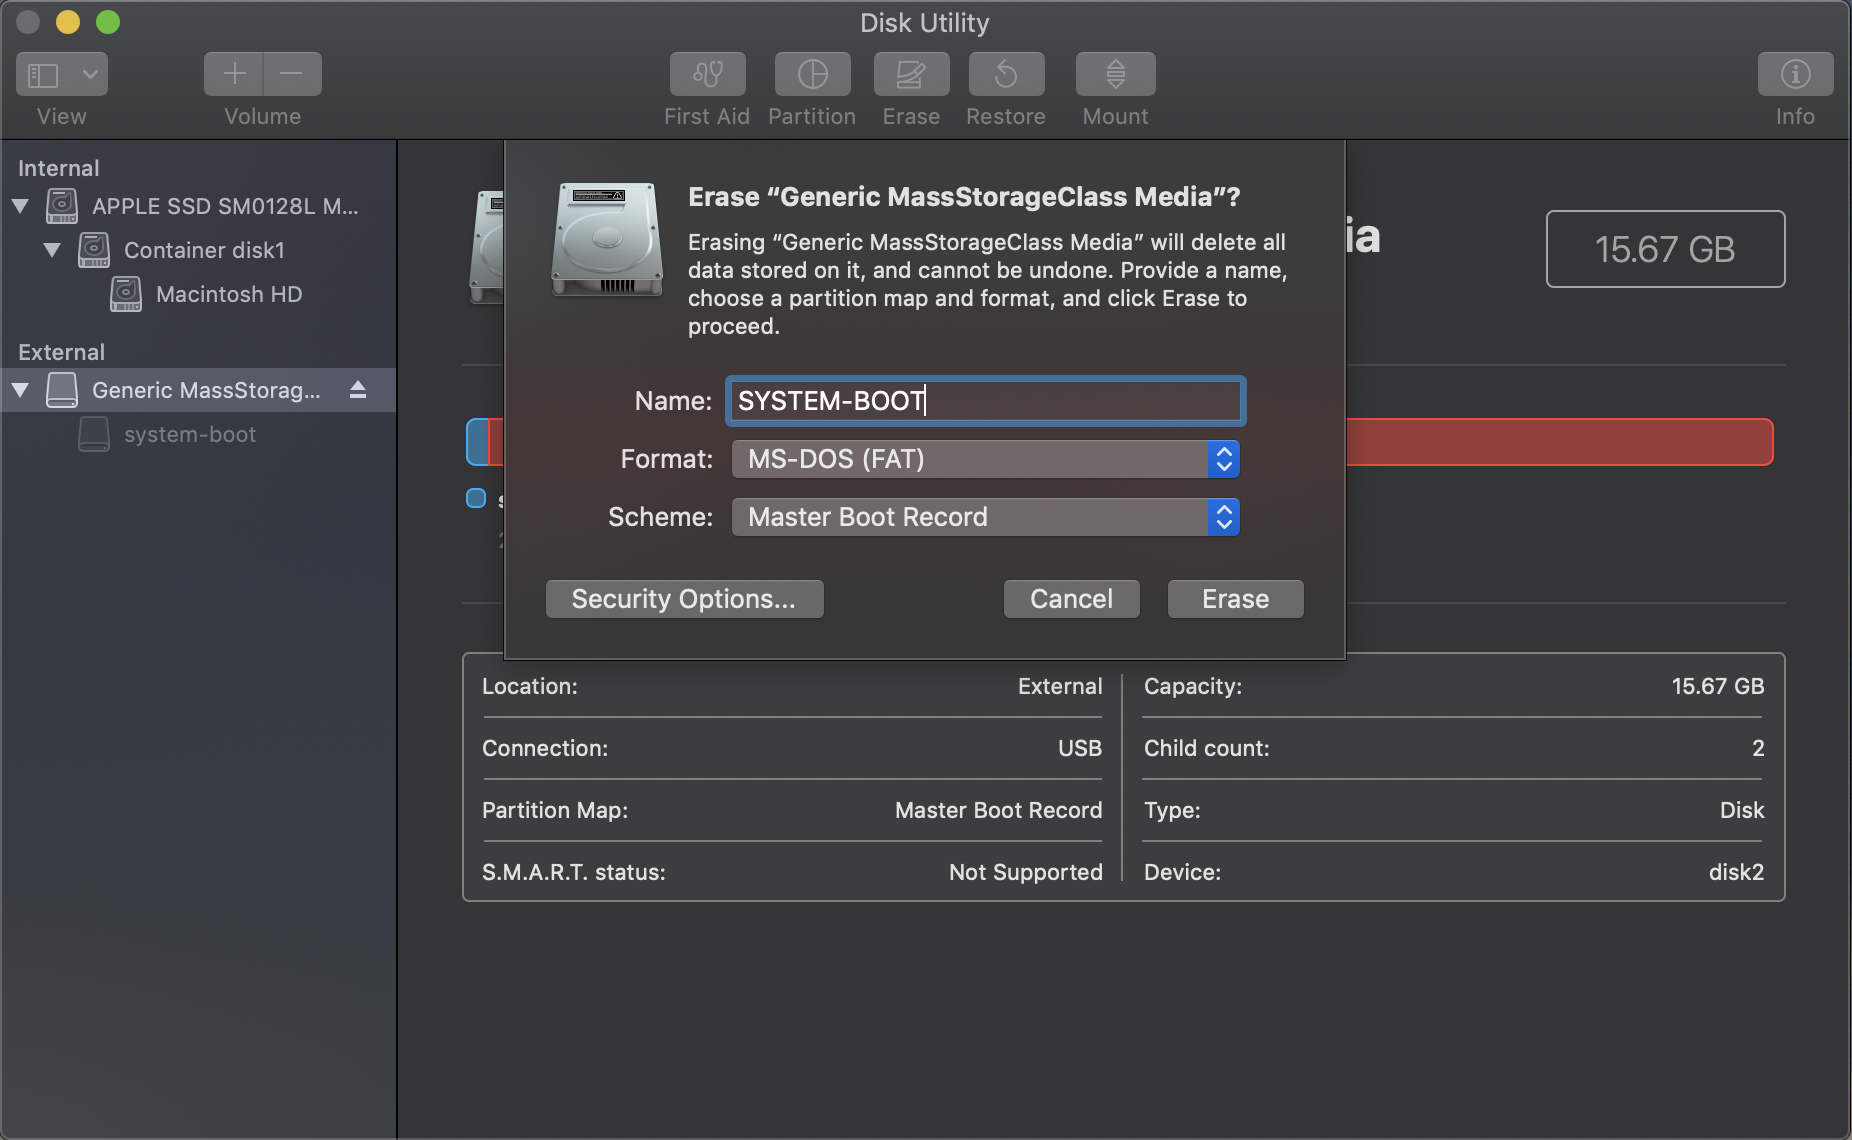
\includegraphics[scale=.3]{Capitulo5/images/format.png}
	\caption{Dando formato a la tarjeta SD}
	\label{fig:formato}
\end{figure} 

Ahora debemos desmontar el volumen y copiar en el la imagen descargada, para conocer el nombre del volumen de la memoria usamos el comando \hl{diskutil list}, buscando la ruta con el nombre de nuestro volumen y lo desmontamos con el comando \hl{diskutil unmountDisk rutaVolumen} el resultado de estos dos comandos se muestra en la figura \ref{fig:desmonataje}.

\begin{figure}[H]
	\centering
	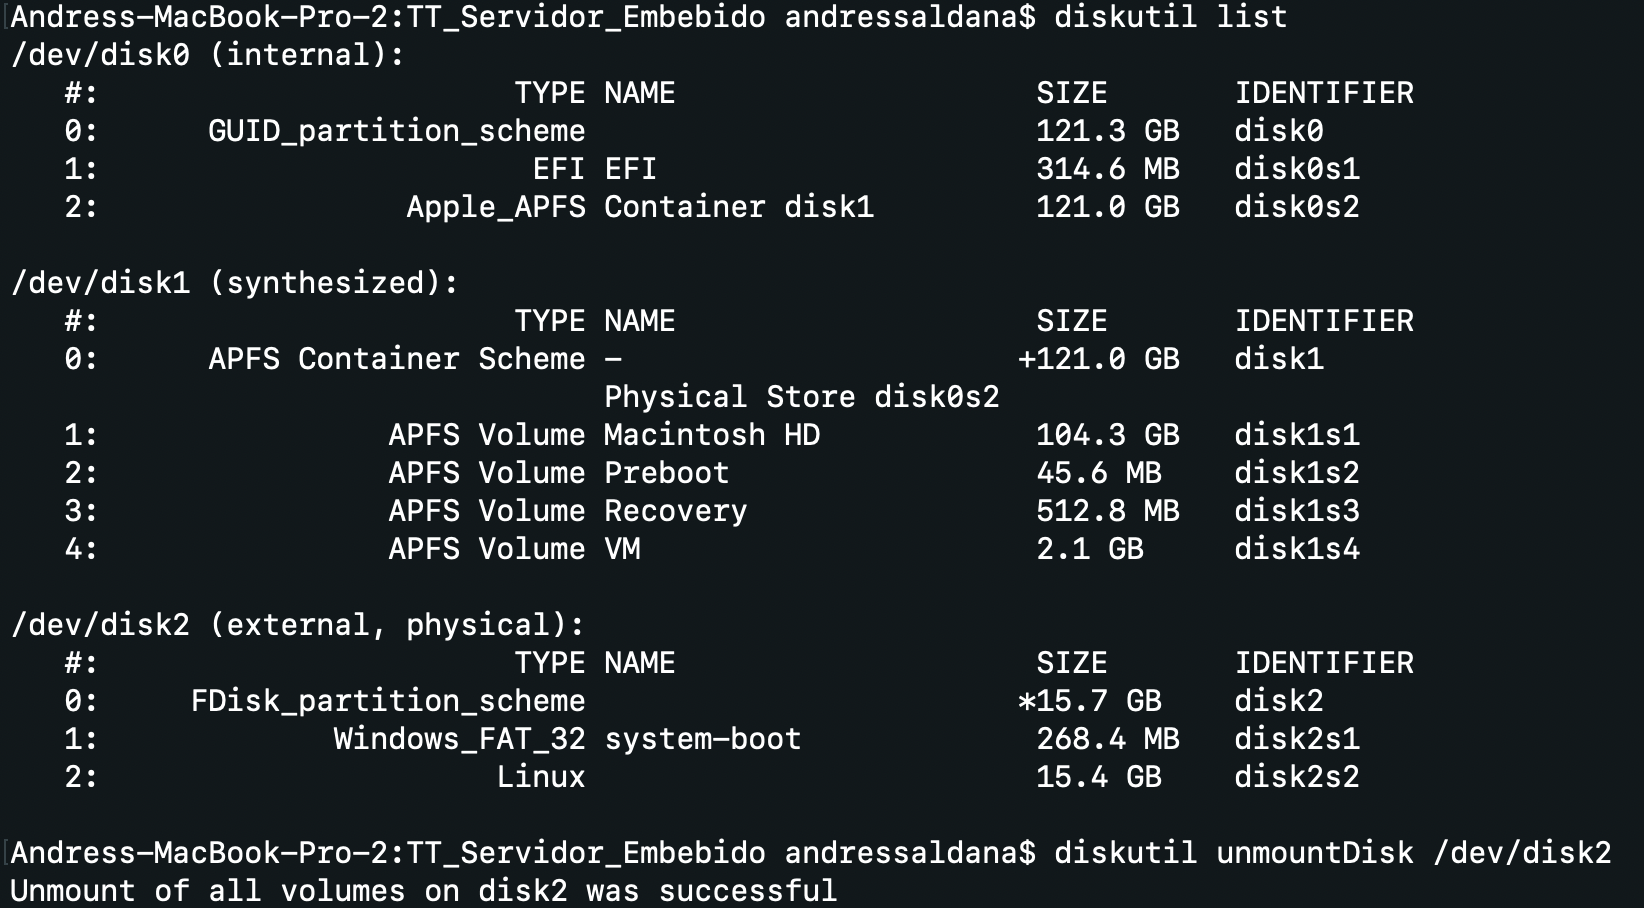
\includegraphics[scale=.4]{Capitulo5/images/unmount.png}
	\caption{Desmontando volumen de memoria SD}
	\label{fig:desmonataje}
\end{figure} 

Copiamos la imagen del sistema operativo a la memoria con el comando \hl{lsudo sh -c 'gunzip -c ~/rutaImagen.img.xz   | sudo dd of=rutaVolumen bs=32m} y nos debe dar una salida en consola como la que se muestra en la figura \ref{fig:copia}.

\begin{figure}[H]
	\centering
	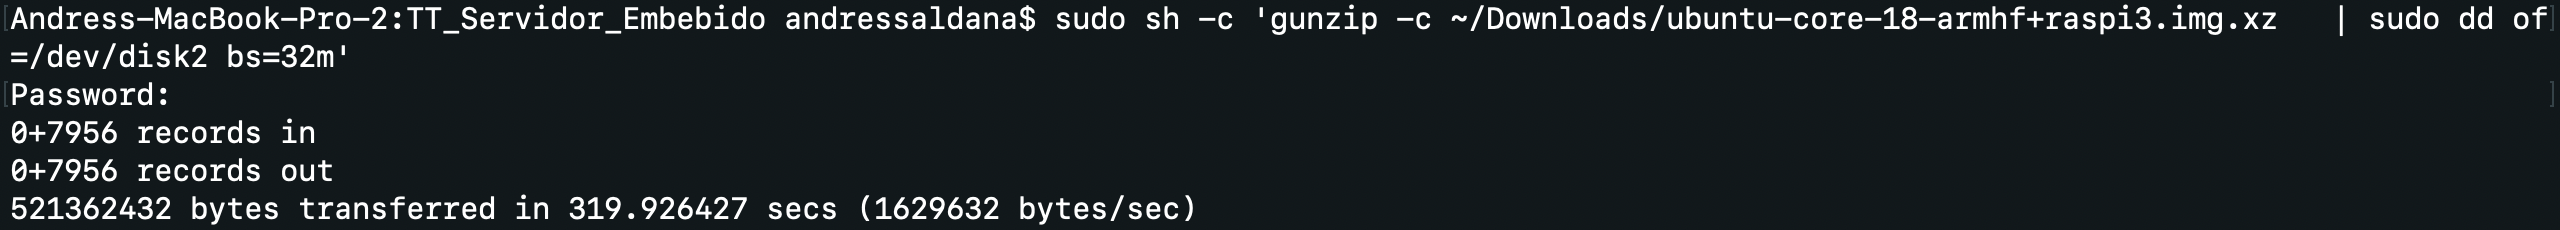
\includegraphics[scale=.3]{Capitulo5/images/copyimg.png}
	\caption{Copiando imagen de sistema operativo a memoria SD}
	\label{fig:copia}
\end{figure} 


Ahora conectamos la Raspberry un monitor con un cable HDMI, un cable ethernet hacia el módem telefónico, un teclado y a la fuente de alimentación como se muestra en la figura \ref{fig:conexion}, debemos crear una cuenta en Ubuntu para asociar un correo electrónico a una llave pública para poder hacer el inicio de sesión remotamente vía ssh, la llave publica se genera con el comando \hl{ssh-keygen -t rsa -b 4096 -C correoasociado@gmail.com} que nos generará dos llaves como se muestra en la figura \ref{fig:llave}, debemos copiar el contenido de la llave pública a el llavero de Ubuntu en su página como se muestra en la figura \ref{fig:ubuntullave}, finalmente, el sistema embebido nos mostrará un mensaje como el de la figura \ref{fig:primer arranque} con el que nos indicara como iniciar sesion vía SSH, ingresando ese comando en una computadora podemos acceder al sistema embebido remotamente \ref{fig:login} 

\begin{figure}[H]
	\centering
	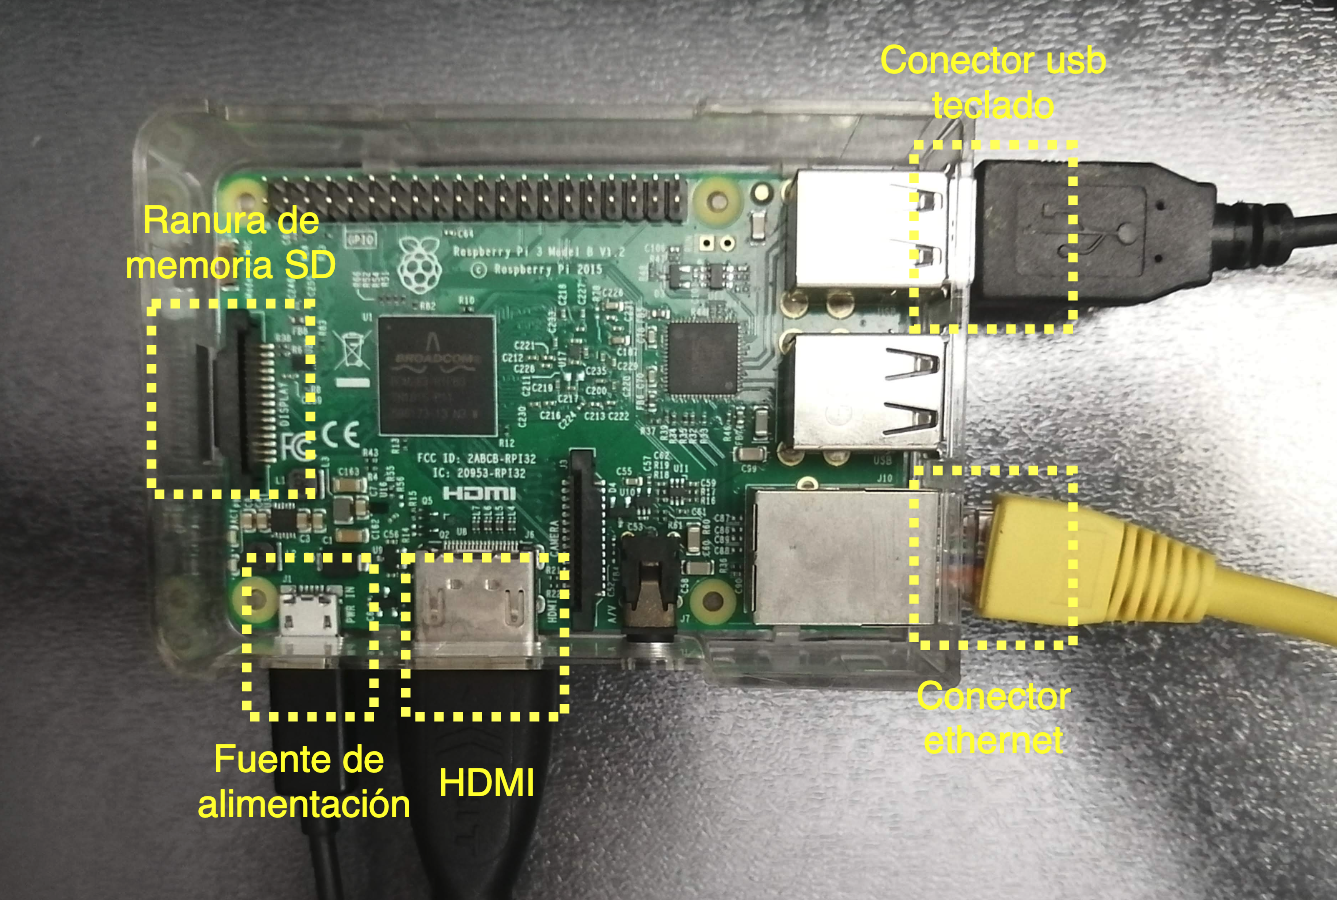
\includegraphics[scale=.25]{Capitulo5/images/rasp.png}
	\caption{Conexión de Raspberry}
	\label{fig:conexion}
\end{figure} 

\begin{figure}[H]
	\centering
	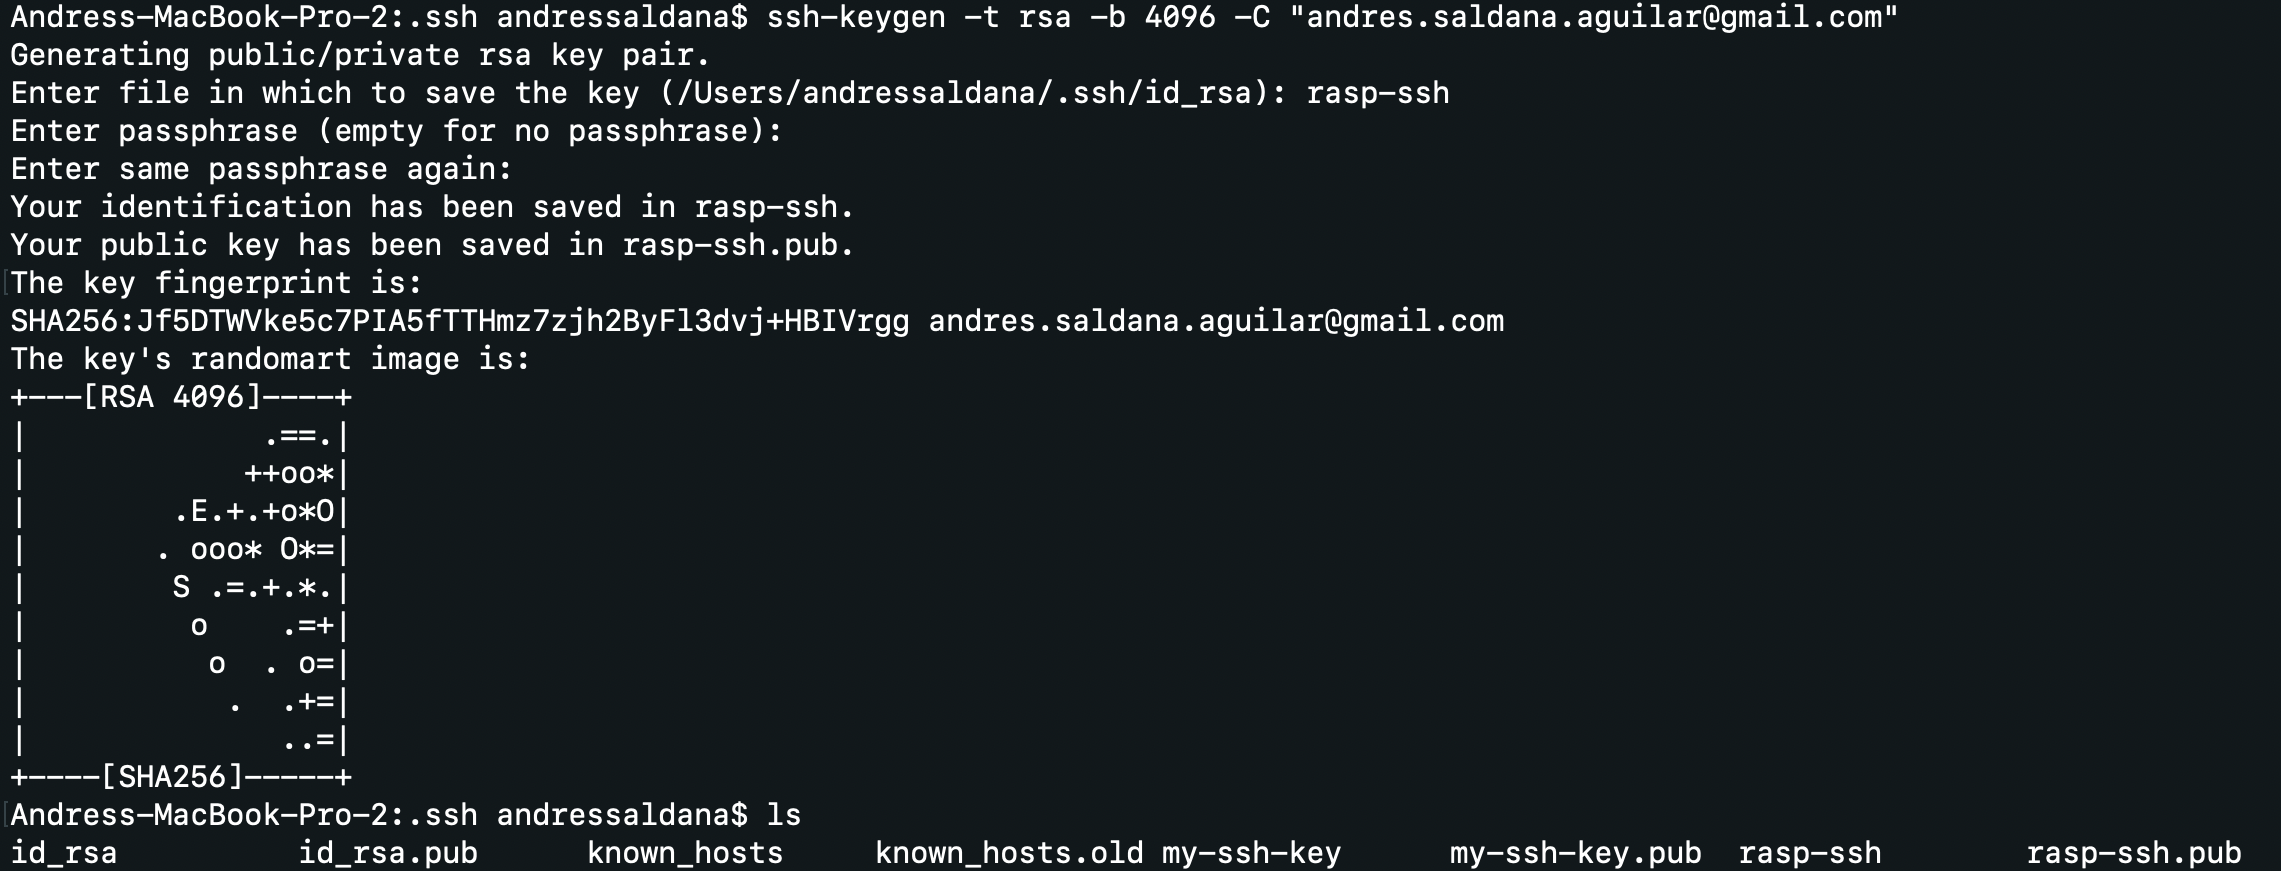
\includegraphics[scale=.3]{Capitulo5/images/ssh_keygen.png}
	\caption{Generando llave pública}
	\label{fig:llave}
\end{figure} 

\begin{figure}[H]
	\centering
	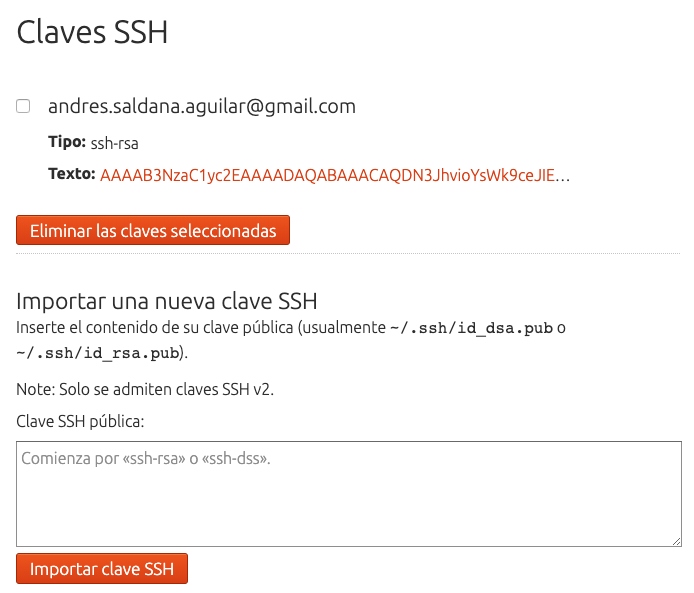
\includegraphics[scale=.3]{Capitulo5/images/sshkey.png}
	\caption{Agregando la llave pública a la cuenta asociada a Ubuntu}
	\label{fig:ubuntullave}
\end{figure} 

\begin{figure}[H]
	\centering
	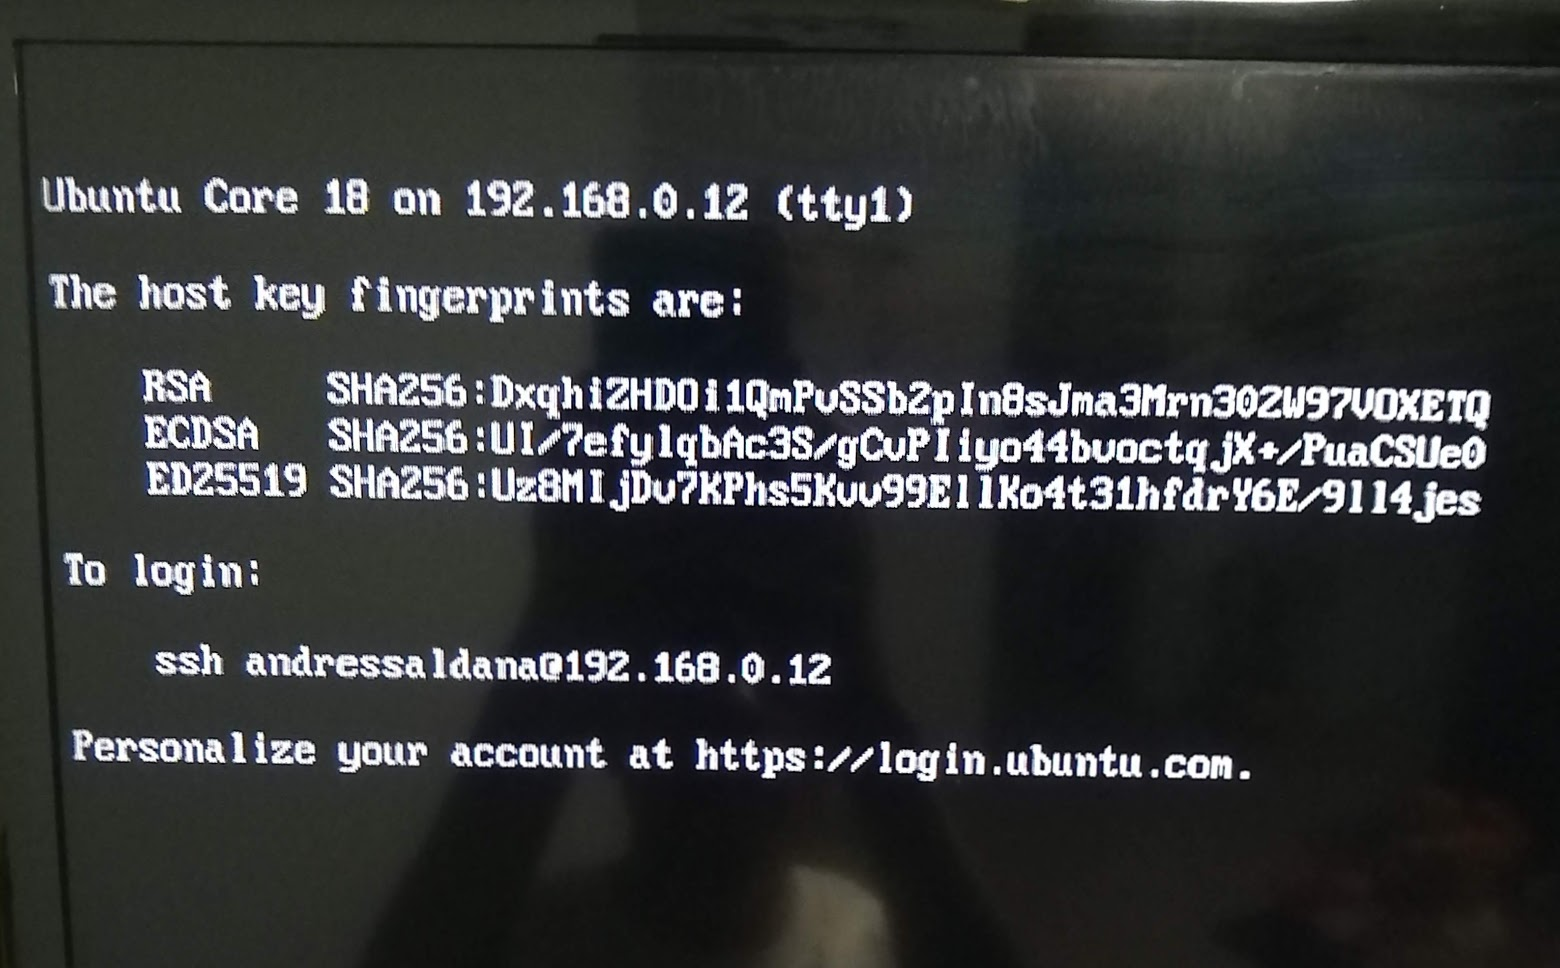
\includegraphics[scale=.15]{Capitulo5/images/first_boot.jpg}
	\caption{Primer arranque del sistema listo para ser utilizado}
	\label{fig:primer arranque}
\end{figure} 

\begin{figure}[H]
	\centering
	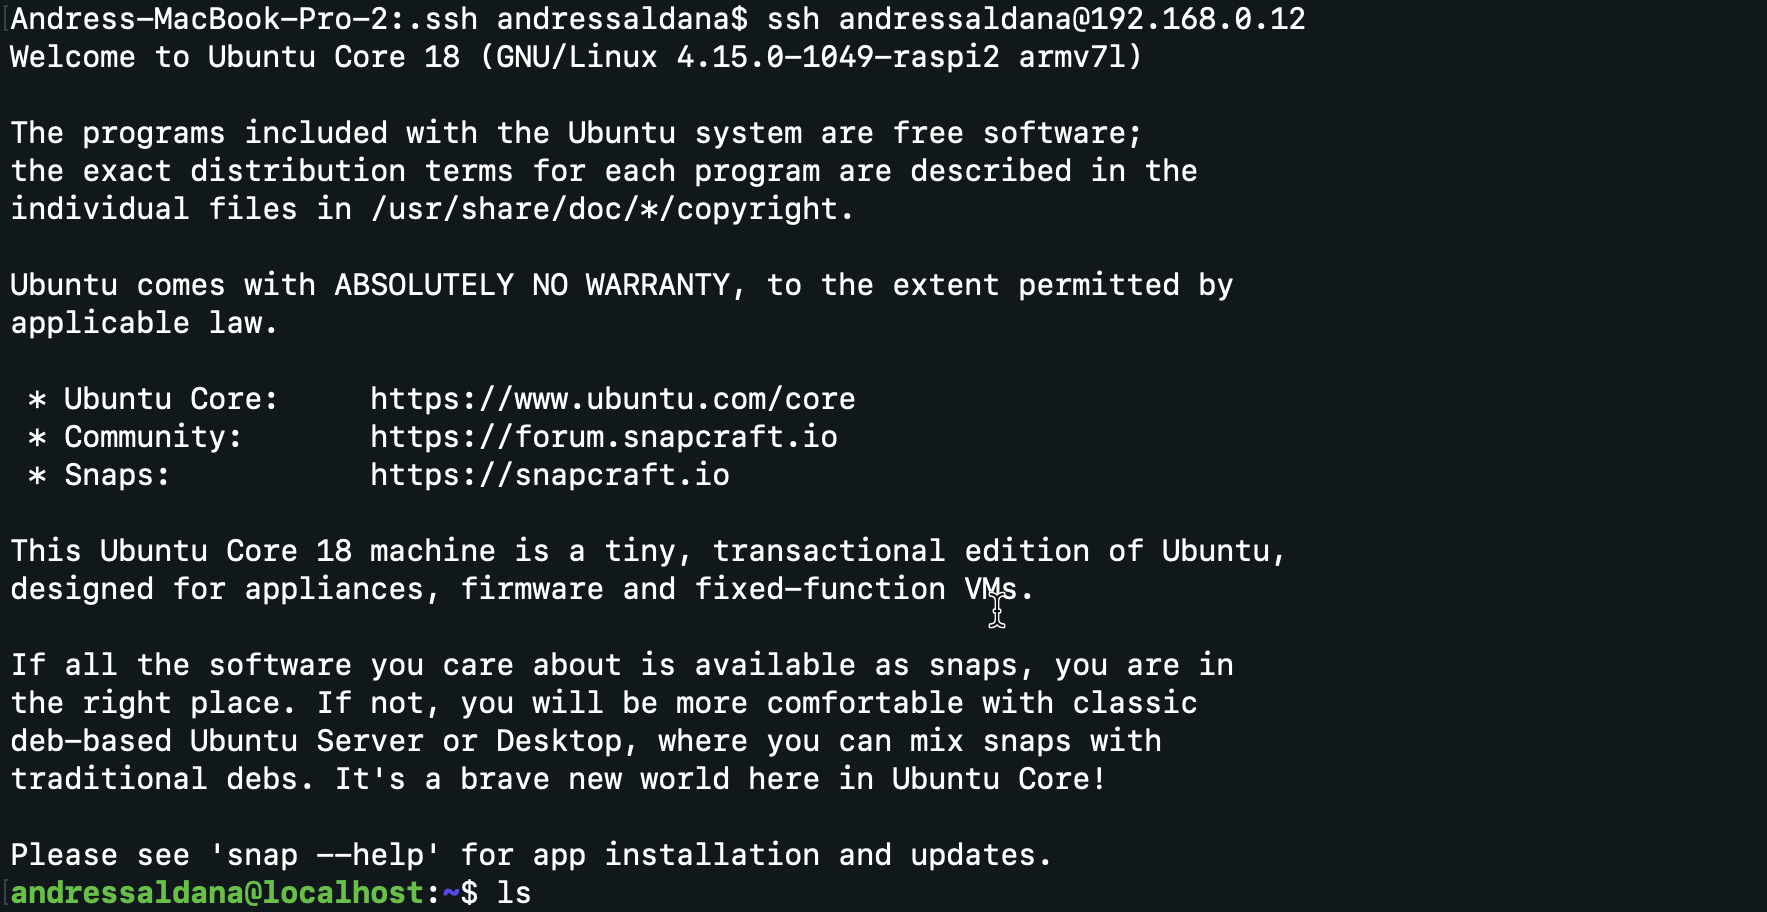
\includegraphics[scale=.3]{Capitulo5/images/login.png}
	\caption{Acceso al servidor embebido de manera remota via SSH}
	\label{fig:login}
\end{figure} 


Con estos pasos, ya tenemos un servidor que es capaz de correr aplicaciones, almacenar hasta 13GB de información en nuestro caso por la capacidad de la memoria SD y con conexión a la red local o inclusive pública si contamos con un proveedor de internet que nos proporcione una IP pública.


\subsection{Creando servicios en Ubuntu Linux}

Todos los programas a implementar serán ejecutados en el sistema embebido como servicios, para ello debemos crear un archivo de configuración por cada uno de los servicios que se ofrecerán con el comando \hl{sudo vi /lib/systemd/system/nombreServicio.service} en el que escribiremos la siguiente configuración:

\begin{lstlisting}
[Unit]
Description=Dummy Service
After=multi-user.target
Conflicts=getty@tty1.service

[Service]
Type=simple
ExecStart=/usr/bin/python3 /direccion/de/programa.py
StandardInput=tty-force

[Install]
WantedBy=multi-user.target
\end{lstlisting}

Reiniciamos el contenedor de demonios del sistema con \hl{sudo systemctl daemon-reload} , habilitamos el servicio que creamos con \hl{sudo systemctl enable nombreServicio.service} e iniciamos su ejecución con \hl{sudo systemctl start nombreServicio.service}.

\subsection{Implementando el servicio de captura y consumo de paquetes UDP provenientes de los microcontroladores}

Este servicio está implementado en el lenguaje de programación Python en su versión 3.0, su propósito es capturar y almacenar en archivos en formato JSON la información proveniente de los sensores de los microcontroladores como indica el caso de uso \ref{SUB-M-CU1.9}, elaboramos un diagrama de flujo para simplificar la explicación de la lógica del programa \ref{fig:programa del servidor microcontrolador}, es importante destacar que estamos usando la técnica de duplicación de procesos (fork en inglés) para duplicar el proceso principal (padre) que conecta y recibe el paquete proveniente de un microcontrolador, delegándole las tareas consecuentes al proceso derivado (hijo), de manera que, el servidor es capaz de conectar más clientes sin tener que perder tiempo en su atención, este programa corre como un servicio en nuestro servidor Linux, es decir, está en ejecución de manera independiente y continua en segundo plano siempre y cuando el servidor no sea reiniciado o apagado.

Para poder identificar bien en el diagrama siguiente que información se esta manipulando, nos apoyamos del modelo de información del servidor embebido  \ref{fig:Base_ServidorEmbebido} enfatizándolo con negritas.

\begin{figure}[H]
	\centering
	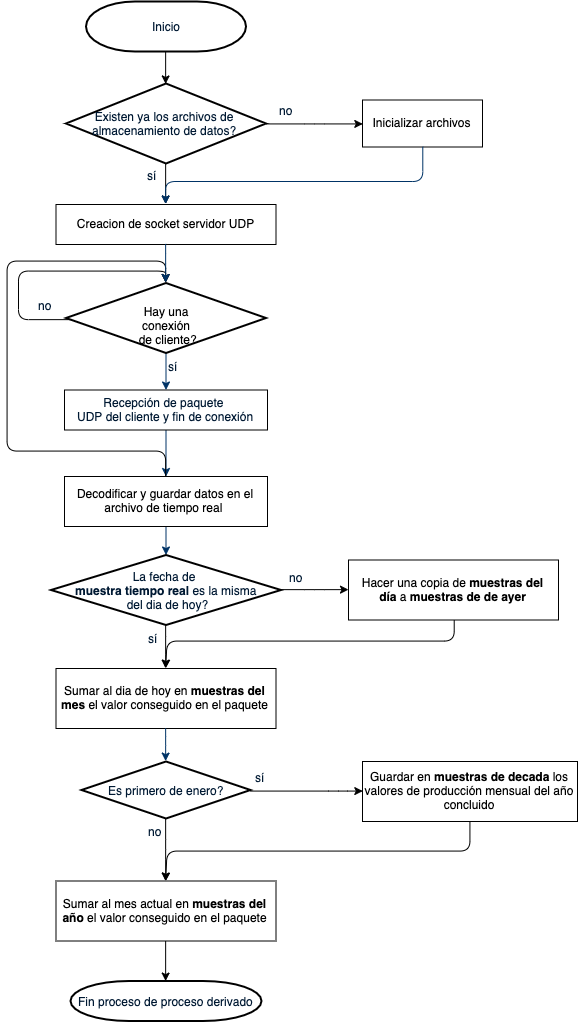
\includegraphics[scale=.5]{Capitulo5/images/logica_server_udp.png}
	\caption{Lógica del programa del servidor del microcontrolador}
	\label{fig:programa del servidor microcontrolador}
\end{figure} 

Para poder comprobar su funcionamiento, redirigimos los paquetes del programa del microcontrolador hacia la IP y puerto 4000 UDP del servidor, teniendo como resultado en consola lo que se muestra en la figura \ref{fig:consola server udp}, donde se muestran las conexiones del microcontrolador, estos mensajes llegan aproximadamente cada segundo más décimas de segundo.

\begin{figure}[H]
	\centering
	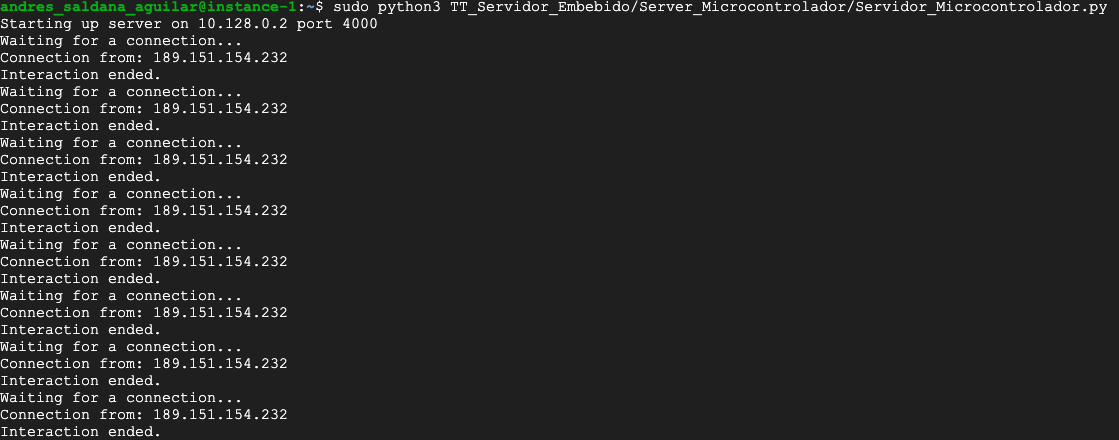
\includegraphics[scale=.3]{Capitulo5/images/udp_server_console.png}
	\caption{Salida de consola del servicio servidor UDP}
	\label{fig:consola server udp}
\end{figure} 

Los archivos que consume este servicio dan como resultado lo mostrado en las siguientes imágenes.

\begin{figure}[H]
	\centering
	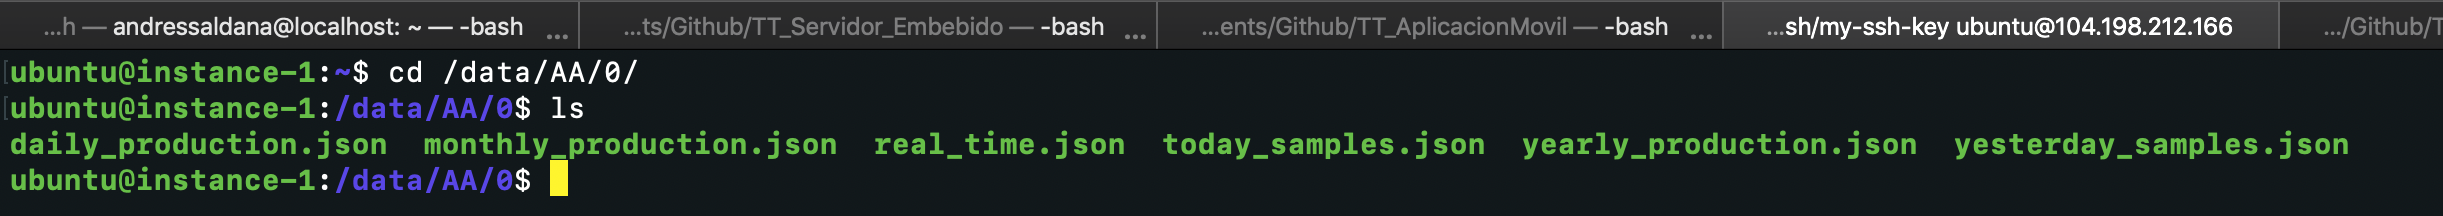
\includegraphics[scale=.3]{Capitulo5/images/dirlist.png}
	\caption{Listado de archivos creados por el servicio de de captura}
	\label{fig:}
\end{figure} 

\begin{figure}[H]
	\centering
	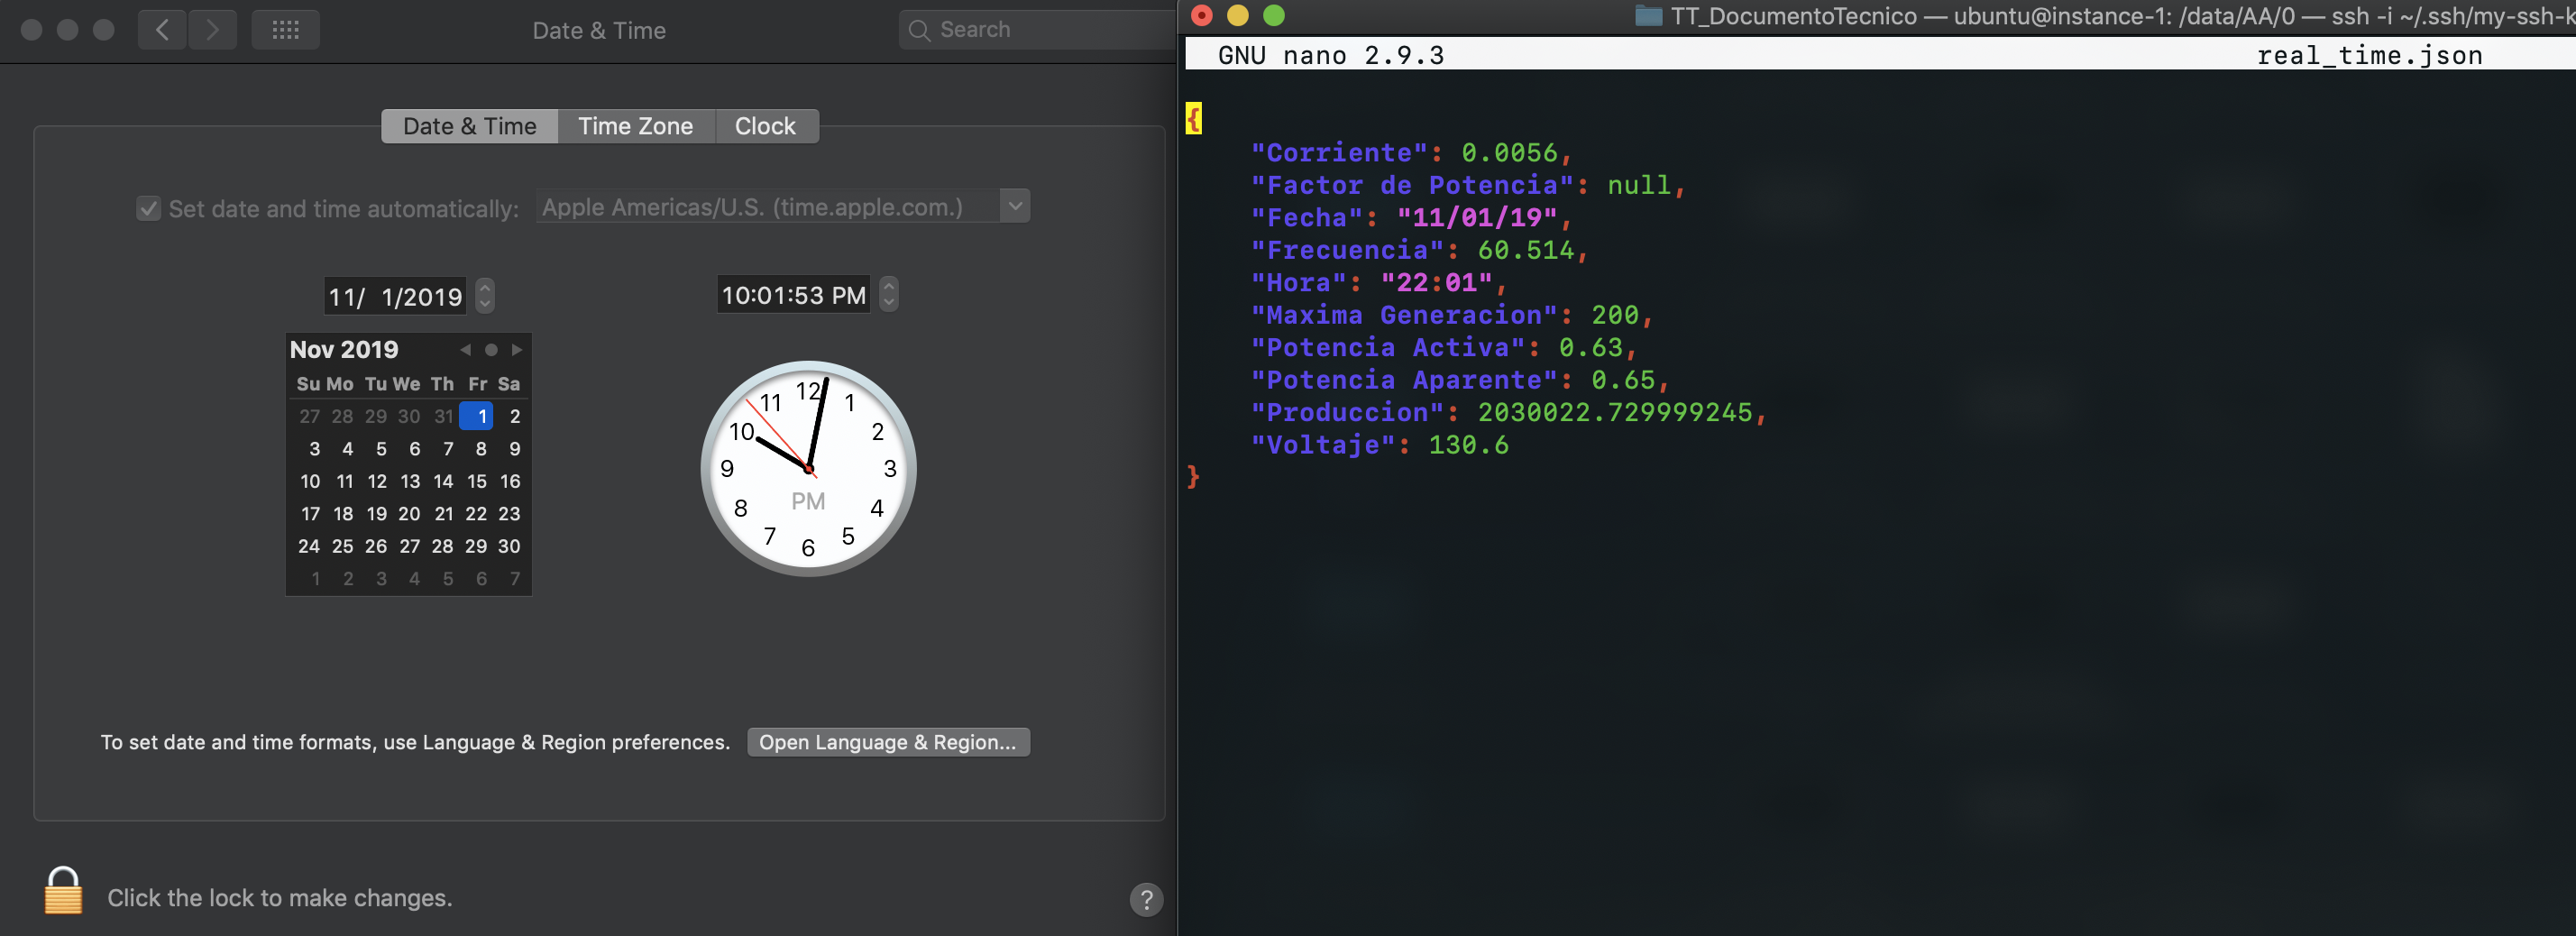
\includegraphics[scale=.3]{Capitulo5/images/real_time.png}
	\caption{Archivo con la muestra de tiempo real}
	\label{fig:}
\end{figure} 

\begin{figure}[H]
	\centering
	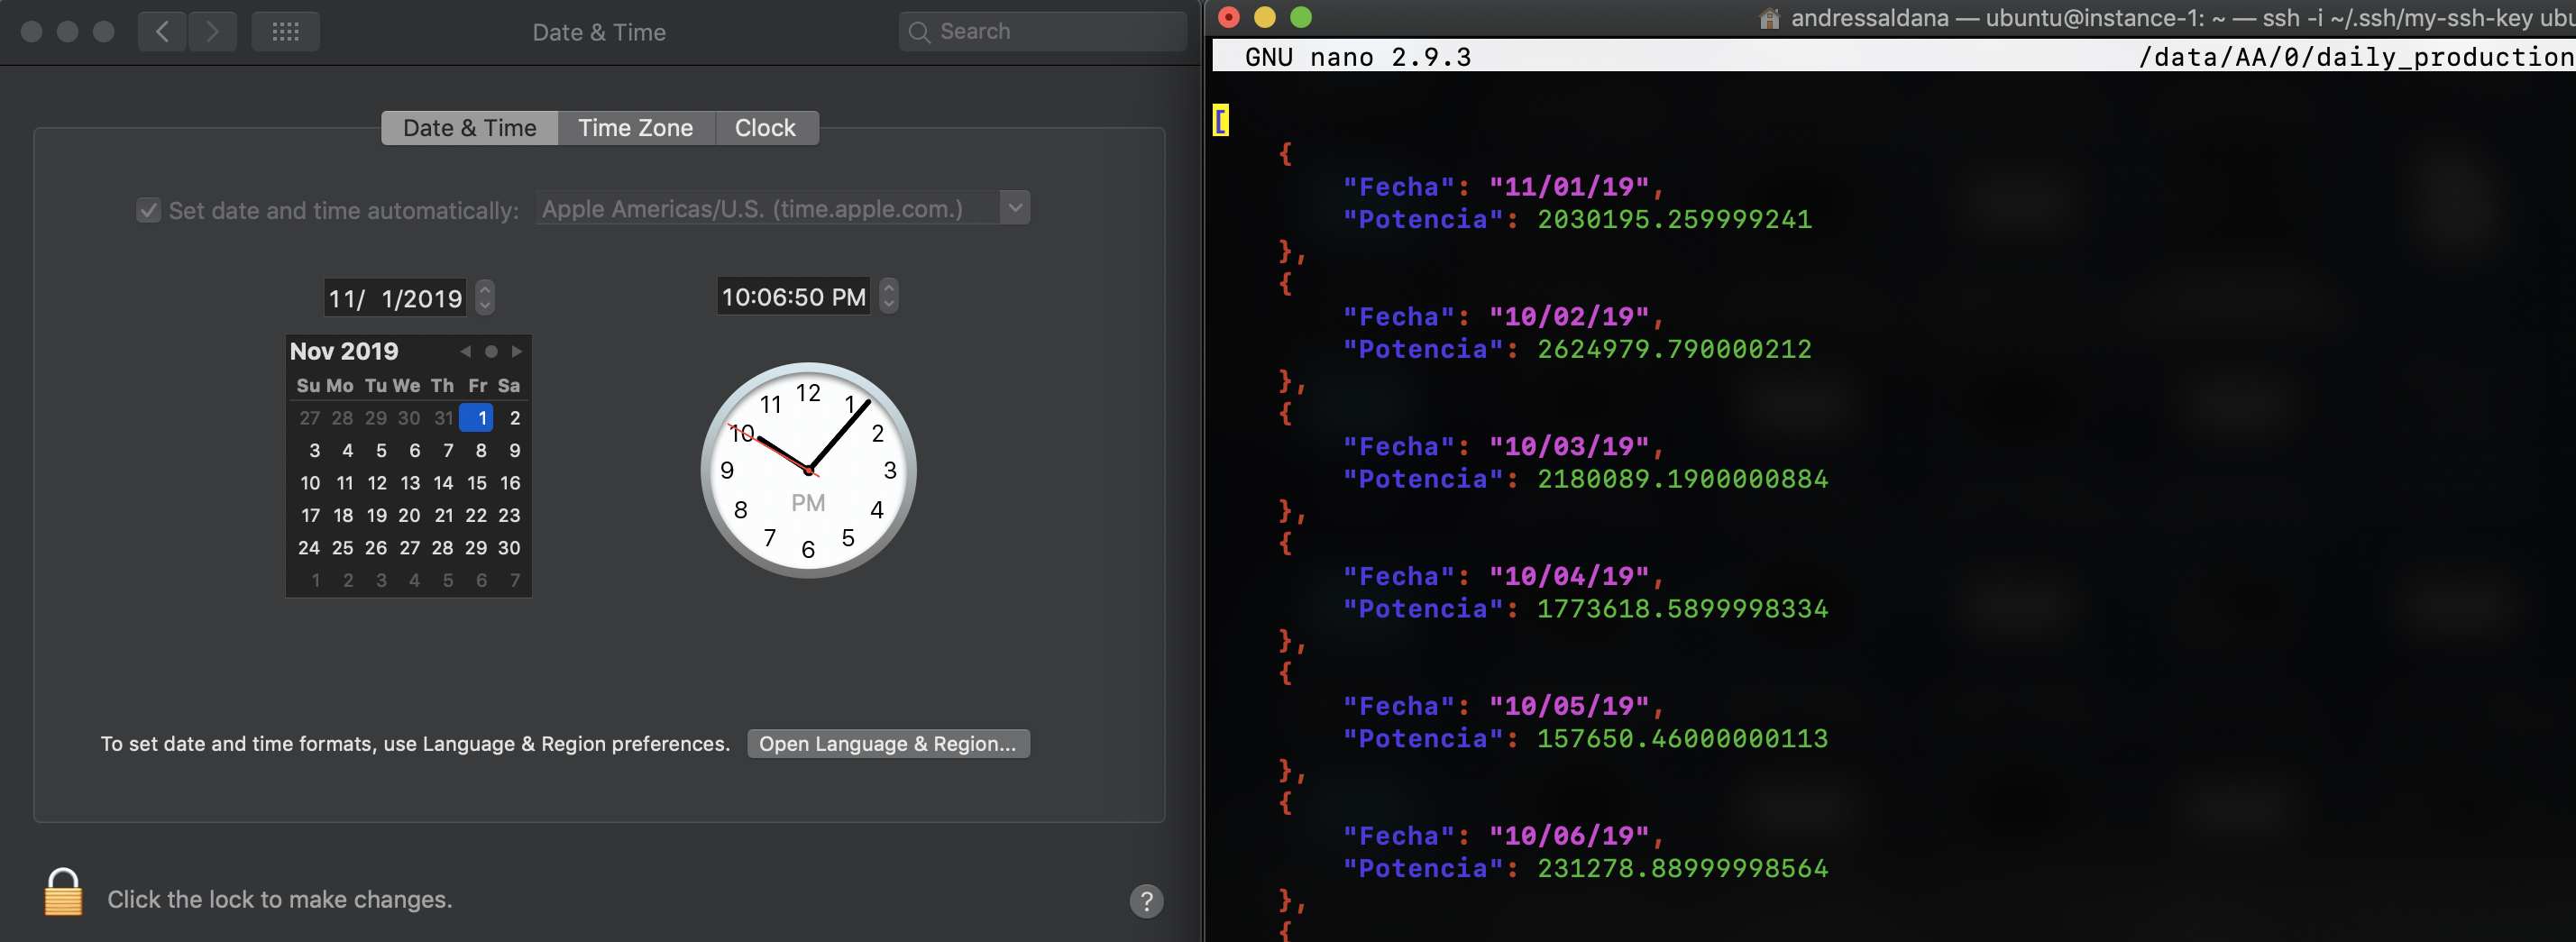
\includegraphics[scale=.3]{Capitulo5/images/daily.png}
	\caption{Extracto de las 31 muestras de producción de energía acumulada por cada día de un mes}
	\label{fig:}
\end{figure}

\begin{figure}[H]
	\centering
	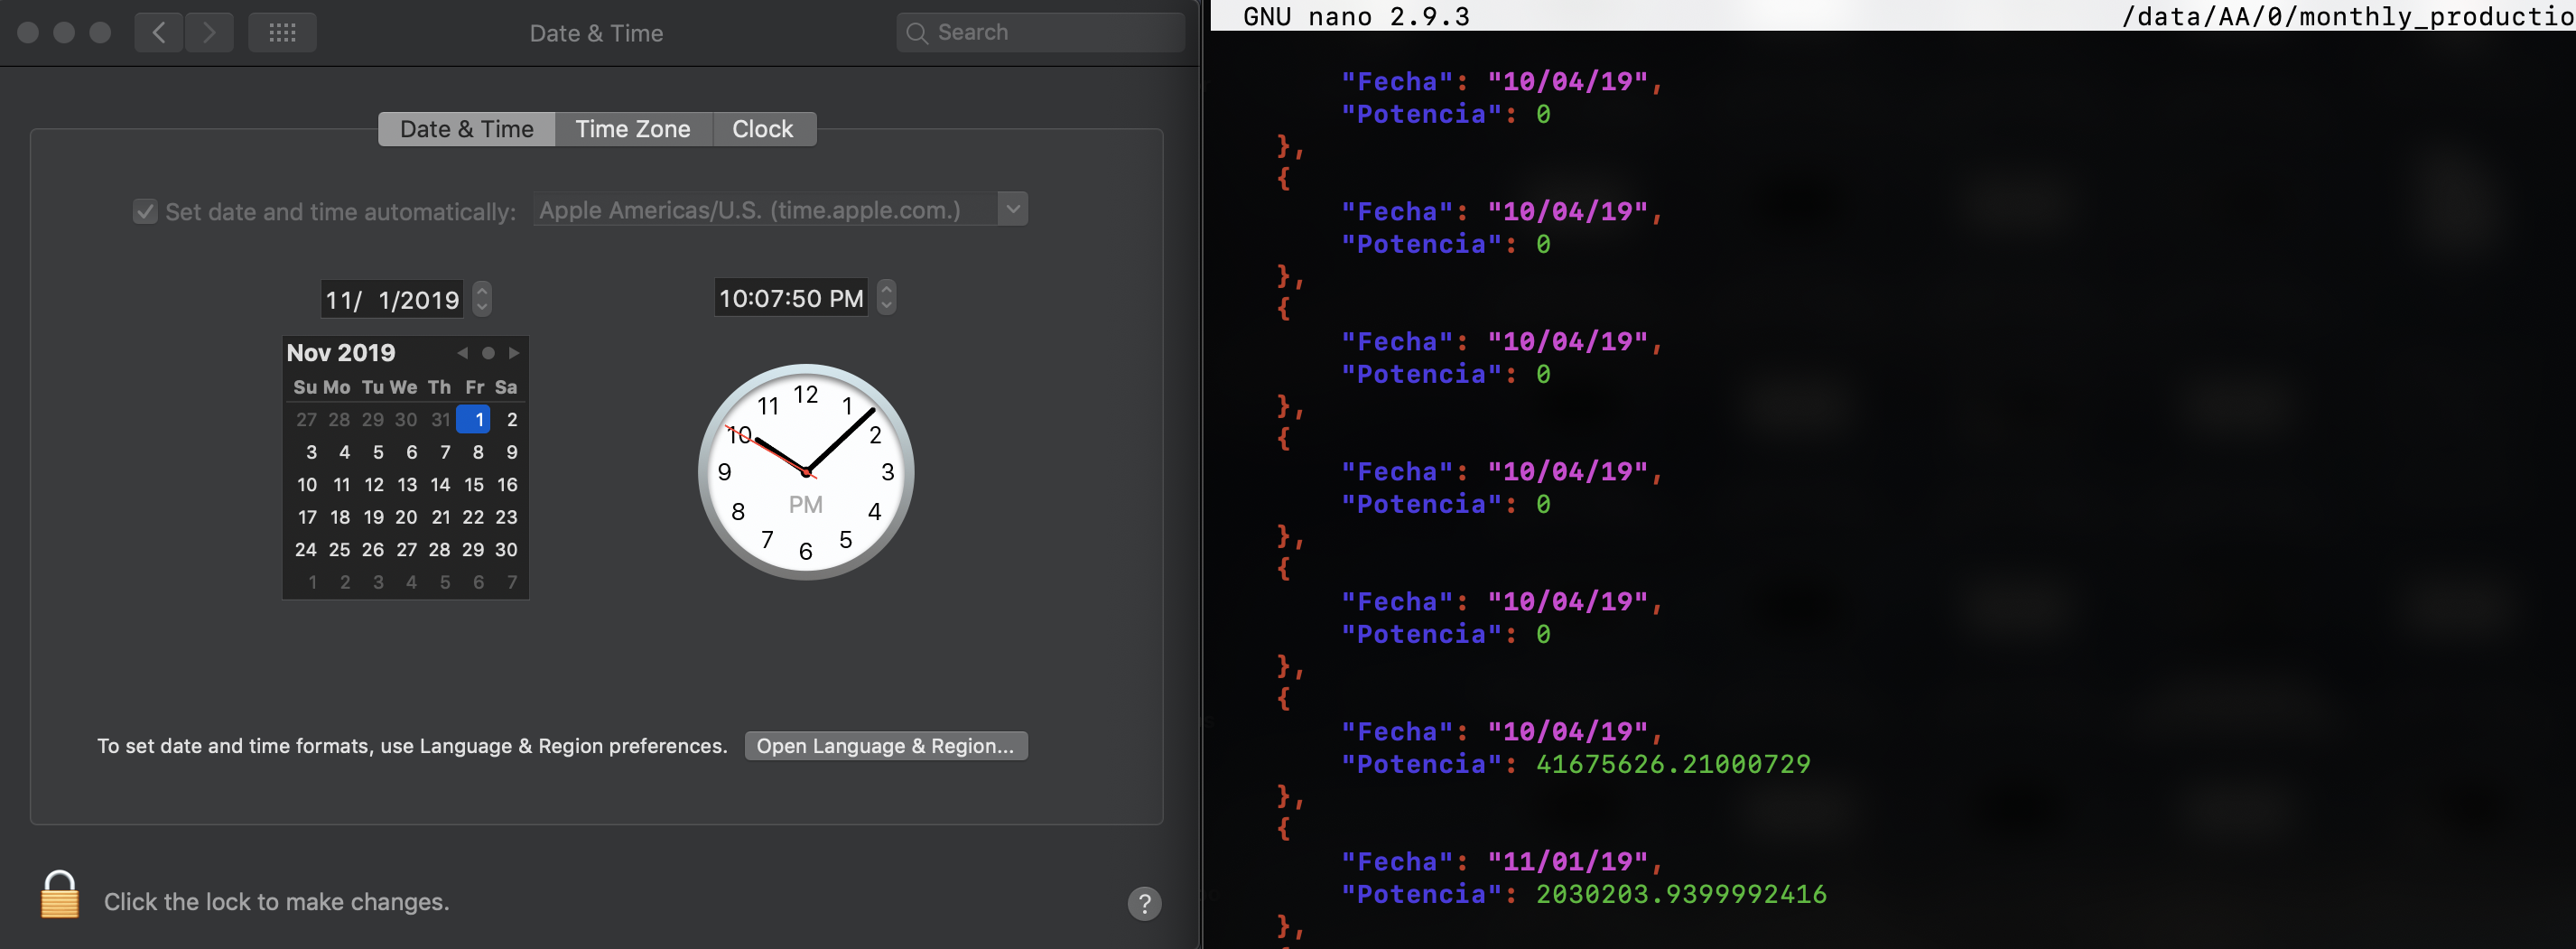
\includegraphics[scale=.3]{Capitulo5/images/monthly.png}
	\caption{Extracto de las 12 muestras de producción de energía acumulada por cada mes del año}
	\label{fig:}
\end{figure} 


\begin{figure}[H]
	\centering
	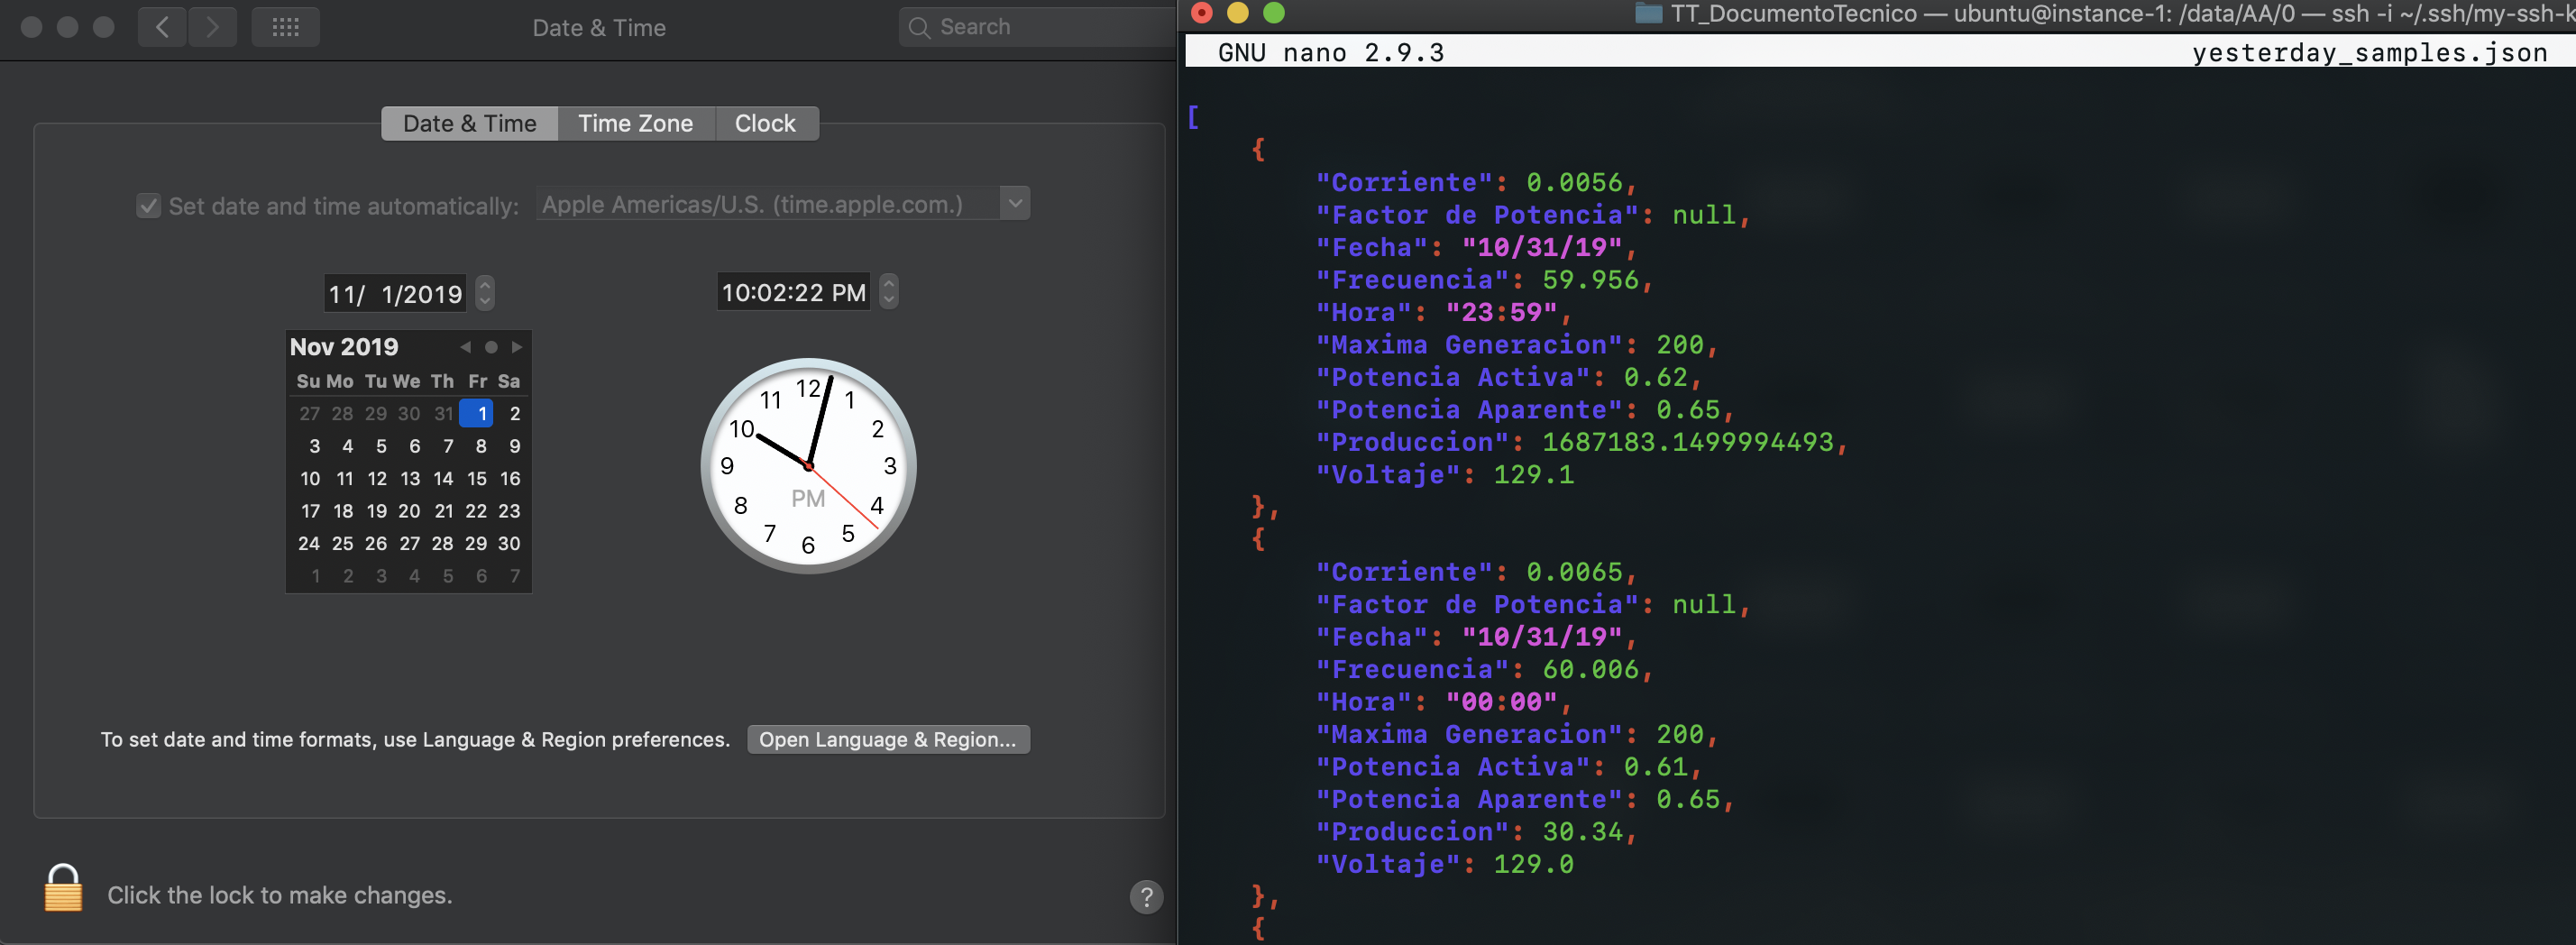
\includegraphics[scale=.3]{Capitulo5/images/yesterday.png}
	\caption{Extracto del archivo de 1440 con las muestras de producción de energía para la gráfica de cada minuto del día de ayer}
	\label{fig:}
\end{figure} 

A continuación, se realizaron pruebas de estrés al servicio para conocer que tanta carga soporta una instancia del servidor


\subsection{Implementando el servicio de creación de gráficas del día actual}

Identificamos que lo mas conveniente sería independizar este proceso de la captura de paquetes para con el propósito de modularizar el sistema y lograr un bajo acoplamiento, implementando la lógica como se muestra en la figura \ref{fig:programa graficador}, la información de gráficas también se guarda en formato JSON, que nos permite hacer mas sencillo la compatibilidad con distintos lenguajes.

\begin{figure}[H]
	\centering
	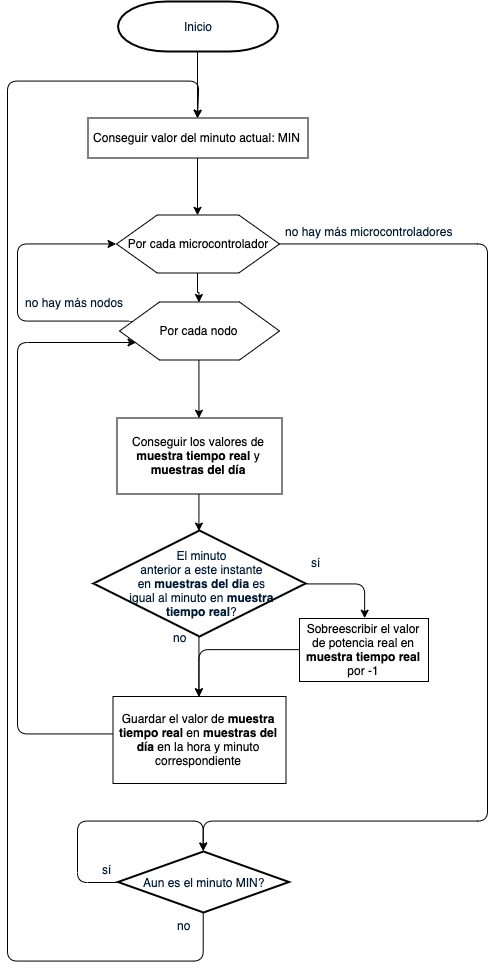
\includegraphics[scale=.5]{Capitulo5/images/logica_graficador.png}
	\caption{Lógica del programa graficador}
	\label{fig:programa graficador}
\end{figure} 

El resultado de este programa se ve reflejado en los archivos de muestras diarias, como se muestra en la figura \ref{fig:muestras diarias}.

\begin{figure}[H]
	\centering
	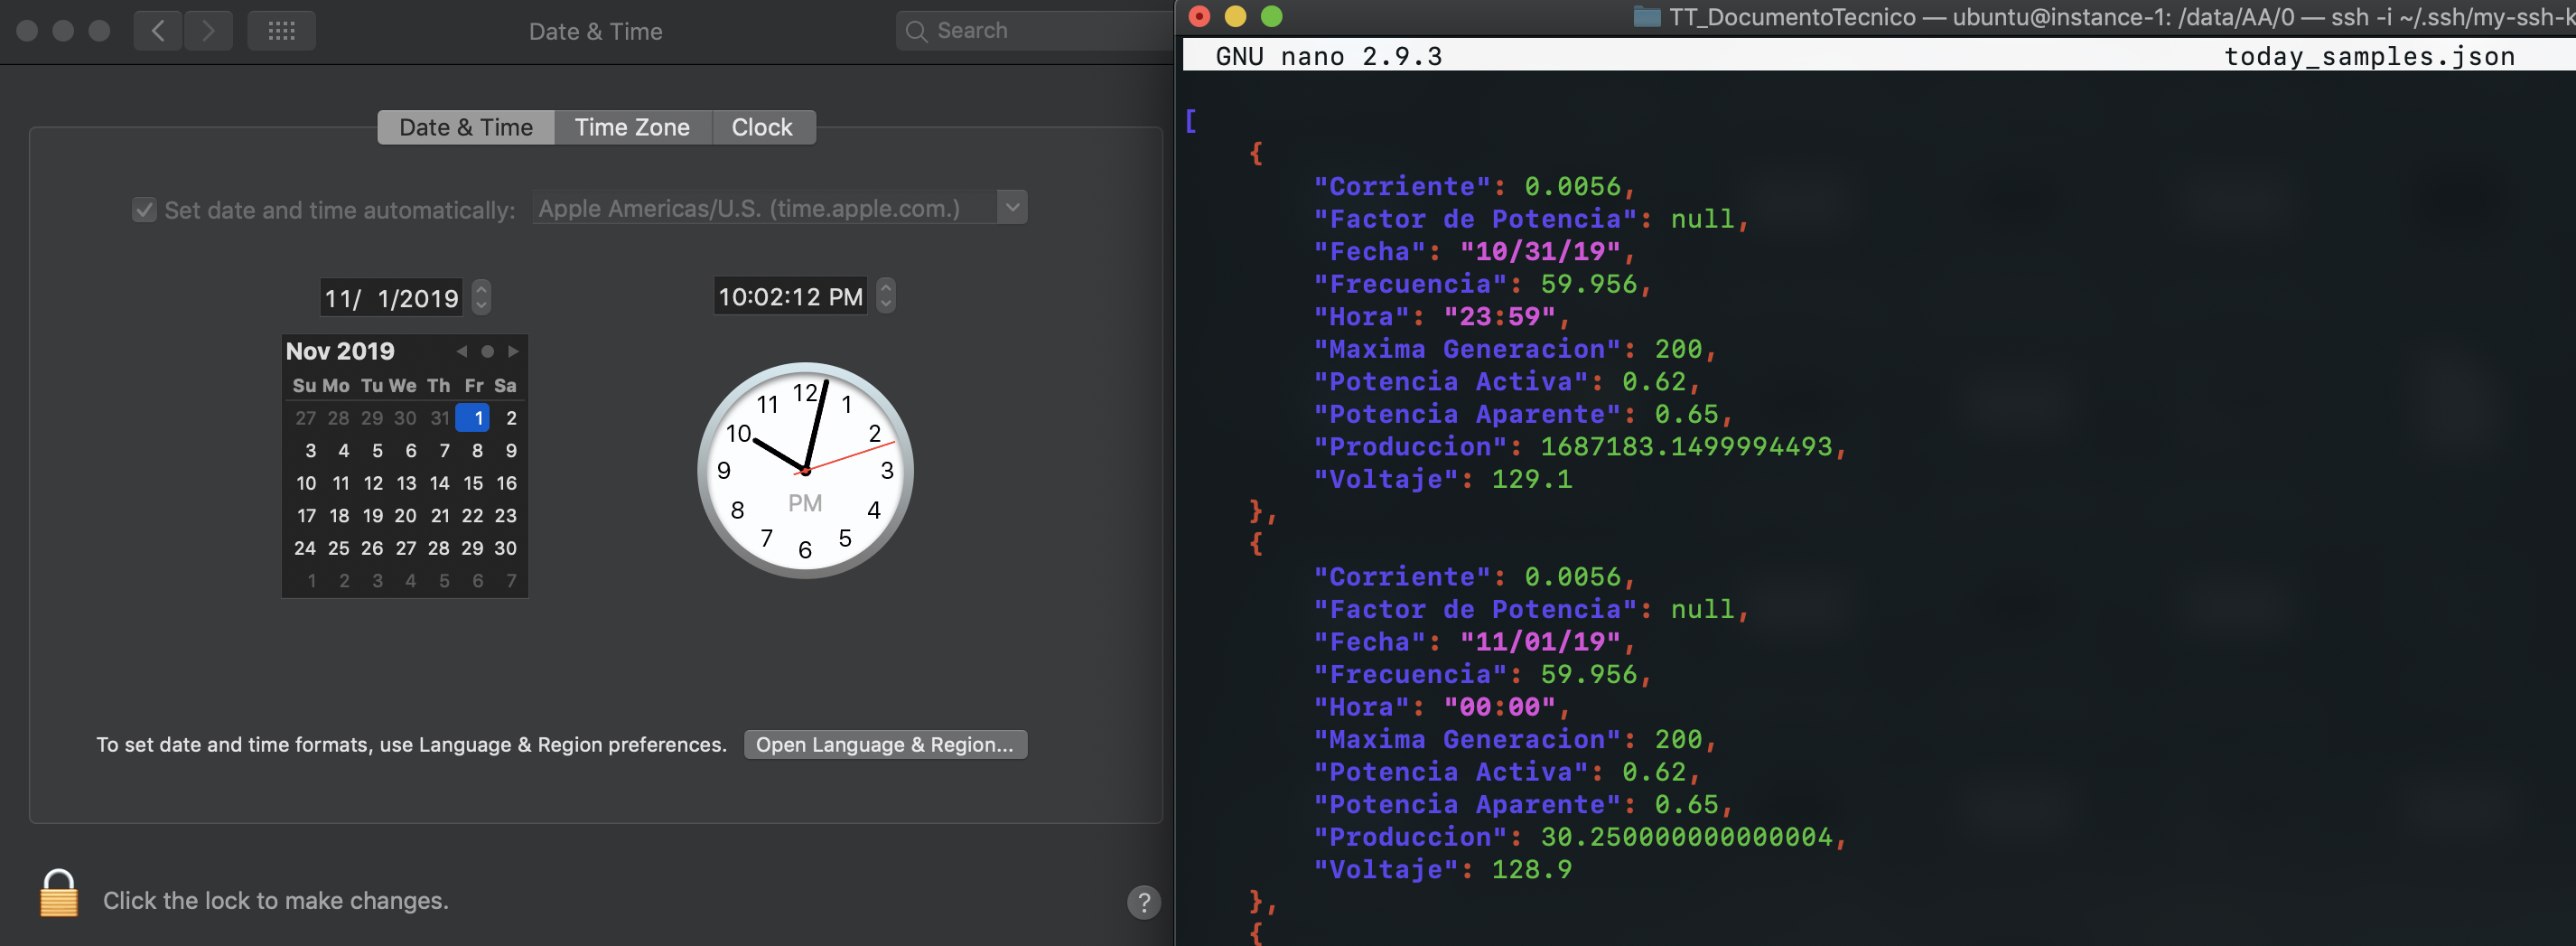
\includegraphics[scale=.3]{Capitulo5/images/today.png}
	\caption{Extracto del archivo de 1440 con las muestras de producción de energía para la gráfica de cada minuto del día de hoy}
	\label{fig:muestras diarias}
\end{figure} 

\subsection{Implementando el servicio de atención a clientes de aplicación móvil}

Este servicio esta implementado en el lenguaje de programación Python en su versión 3.0, su propósito es atender las peticiones provenientes de la aplicación móvil como indica el caso de uso \ref{SUB-M-CU1.10}, elaboramos un diagrama de flujo para simplificar la explicación de la lógica del programa \ref{fig:programa del servidor aplicacion}, también hicimos uso de la duplicación de procesos para aumentar el rendimiento del programa, este programa corre como un servicio en nuestro servidor Linux.

\begin{figure}[H]
	\centering
	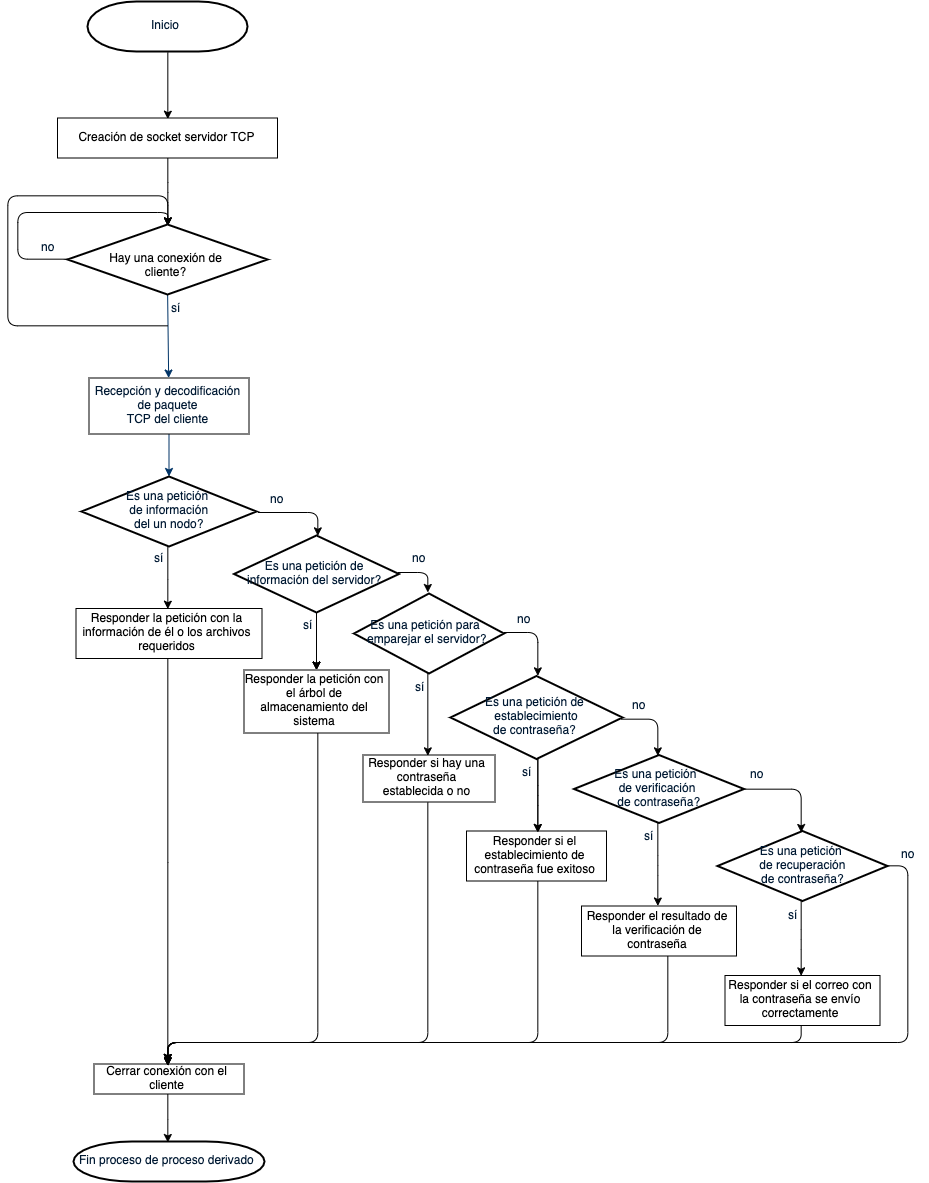
\includegraphics[scale=.4]{Capitulo5/images/logica_server_tcp.png}
	\caption{Lógica del programa del servidor de la aplicación}
	\label{fig:programa del servidor aplicacion}
\end{figure} 

Para probar su funcionamiento, se realizaron las peticiones posibles hacia el servidor:

Comando: \hl{getdata AA 0 realtime}
\begin{figure}[H]
	\centering
	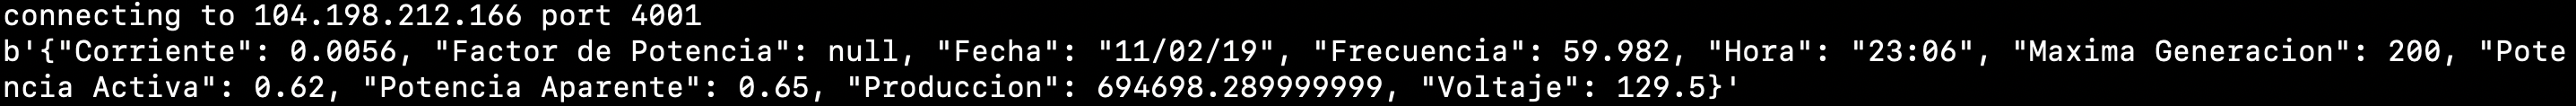
\includegraphics[scale=.3]{Capitulo5/images/get_data.png}
	\caption{Respuesta del comando para conseguir la información del el archivo de tiempo real}
	\label{fig:}
\end{figure} 

Comando: \hl{getinfo}
\begin{figure}[H]
	\centering
	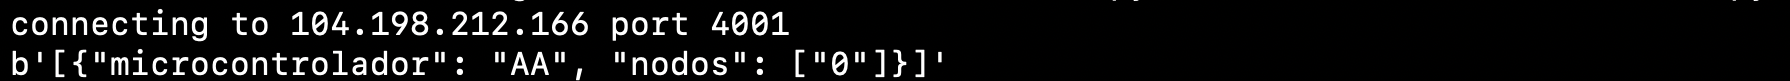
\includegraphics[scale=.5]{Capitulo5/images/get_info.png}
	\caption{Respuesta del comando que trae la información del árbol de información del servidor}
	\label{fig:}
\end{figure} 

Comando: \hl{connect}
\begin{figure}[H]
	\centering
	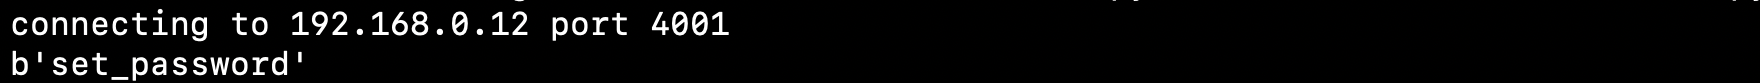
\includegraphics[scale=.5]{Capitulo5/images/connect.png}
	\caption{Respuesta a conocer si el servidor tiene ya una contraseña, nos indica que no hay contraseña}
	\label{fig:}
\end{figure} 

\begin{figure}[H]
	\centering
	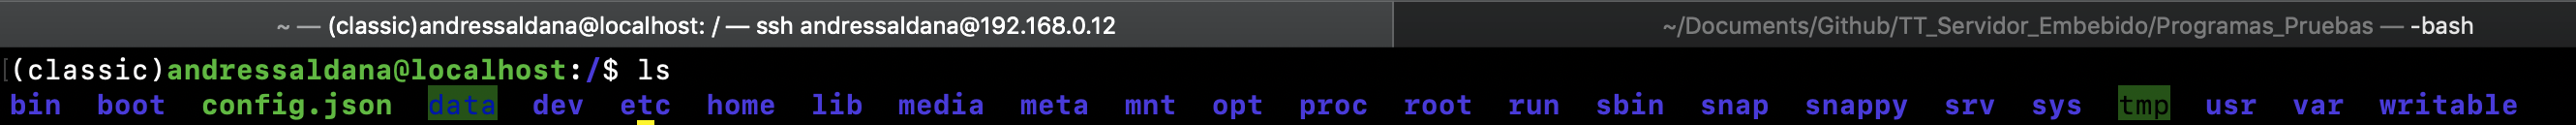
\includegraphics[scale=.35]{Capitulo5/images/listconfig.png}
	\caption{Ubicación del archivo de configuración, en el directorio raíz con el nombre de config.json}
	\label{fig:}
\end{figure} 

\begin{figure}[H]
	\centering
	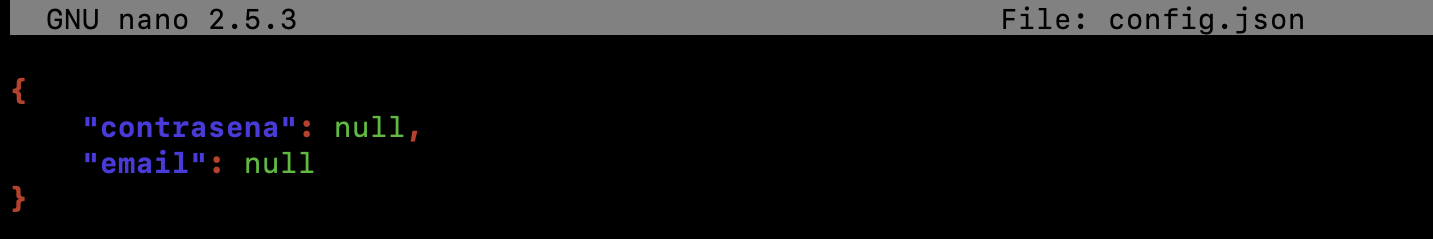
\includegraphics[scale=.5]{Capitulo5/images/nullconfig.png}
	\caption{Archivo de configuración con variables sin asignar}
	\label{fig:}
\end{figure} 

Comando: \hl{setpassword Secret1 smonitorp@gmail.com}
\begin{figure}[H]
	\centering
	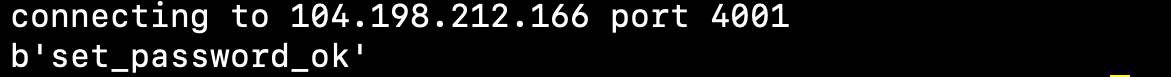
\includegraphics[scale=.5]{Capitulo5/images/set_password.png}
	\caption{Respuesta al comando que configura la contraseña}
	\label{fig:}
\end{figure} 

\begin{figure}[H]
	\centering
	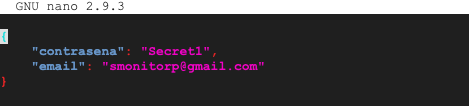
\includegraphics[scale=.6]{Capitulo5/images/setconfig.png}
	\caption{Archivo de configuración con variables asignadas después del setpassword}
	\label{fig:}
\end{figure} 

Comando: \hl{getpassword Secret1}
\begin{figure}[H]
	\centering
	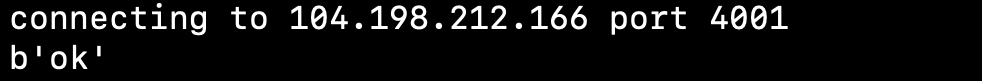
\includegraphics[scale=.5]{Capitulo5/images/forgot_pass.png}
	\caption{Respuesta a verificación de constraseña}
	\label{fig:}
\end{figure} 

Comando: \hl{forgotpassword}
\begin{figure}[H]
	\centering
	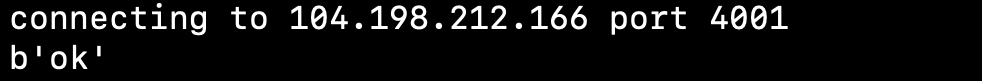
\includegraphics[scale=.5]{Capitulo5/images/forgot_pass.png}
	\caption{Respuesta del envió del correo, 'ok' si es exitoso, 'error' si el envió fue fallido}
	\label{fig:}
\end{figure} 

\begin{figure}[H]
	\centering
	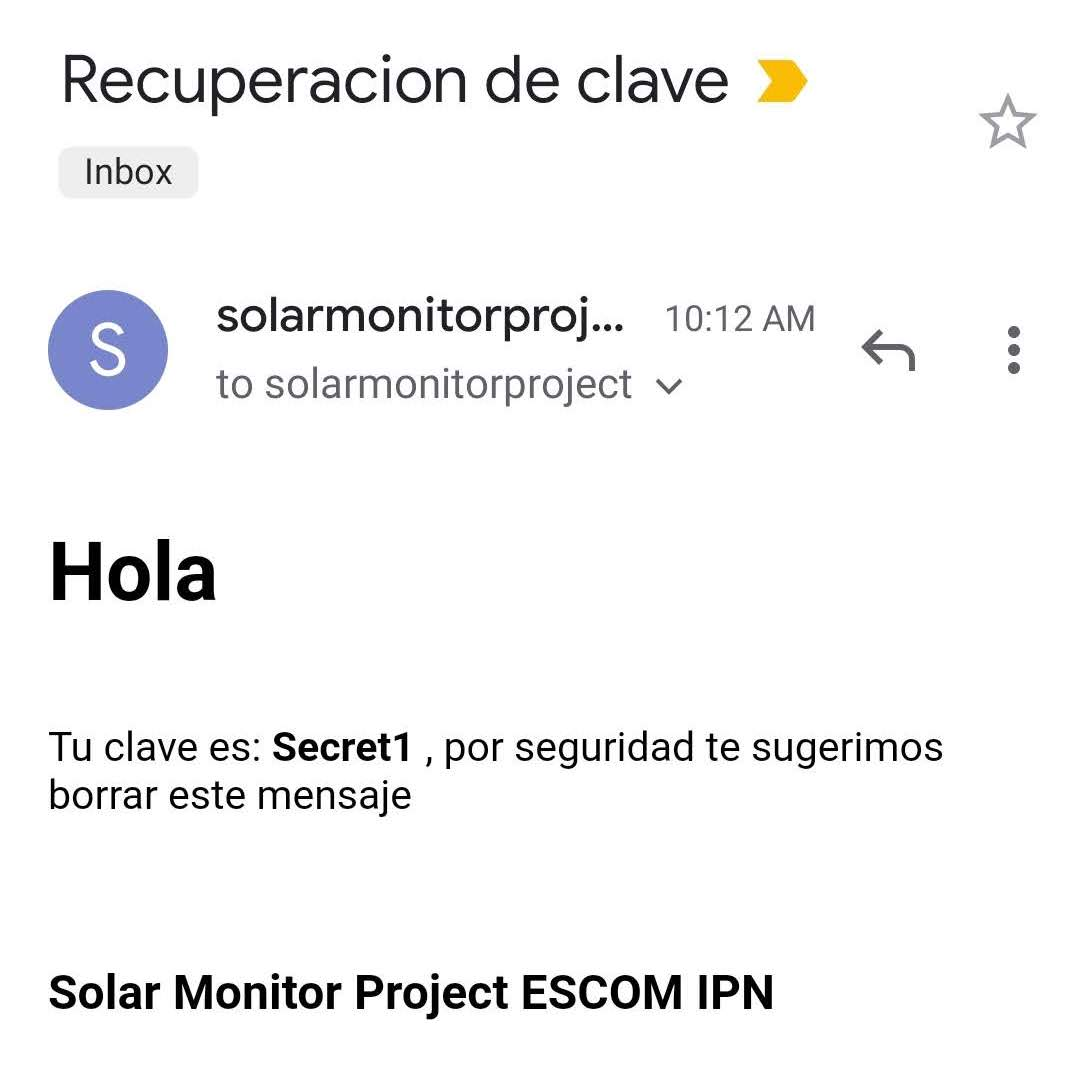
\includegraphics[scale=.2]{Capitulo5/images/correo.jpg}
	\caption{Correo resultado del comando forgotpassword}
	\label{fig:}
\end{figure}

